\section{Results}
\label{sec:results}


\subsection{Local Fractal Dimension of Datasets}
\label{sec:results:lfd-of-datasets}

Since the time complexity of CAKES algorithms scales with the LFD of the dataset, we examine the LFD of each dataset we used for benchmarks.

Figure~\ref{fig:results:lfd-plots} the trends in LFD for (the non-augmented versions of) Fashion-Mnist, Glove-25, Sift, Random, Silva 18S, and RadioML.
The horizontal axis denotes the depth in the cluster tree, and the vertical axis denotes the LFD (as calculated by Equation~\ref{eq:methods:lfd-simplified}) of clusters at that depth.
We plot lines for the 5$^{th}$, 25$^{th}$, 50th, 75$^{th}$ and 95$^{th}$ percentiles of LFD, as well as the minimum and maximum LFD at each depth.
In order to have the plots to best reflect the distribution of LFDs across the entire \emph{dataset}, we compute percentiles counting each cluster as many times as its cardinality.
In other words, if, for some dataset, the 95$^{th}$ percentile of LFD at depth 40 is 3, this means that 95\% of the total points in clusters at depth 40 belong to clusters whose LFD is at most 3.

Figure~\ref{fig:results:fashion-mnist-lfd} shows the LFD by depth for Fashion-Mnist.
We observe that until about depth 5, the LFD is low, as the 95$^{th}$ percentile (orange plotted line) is less than 4, and the median (red line) is just above 2.
For depths 15 through 25, we observe that the LFD increases, with the 95$^{th}$ percentile (orange plotted line) slightly less than 6, and the median near 3.
Finally, for depths 25 through the maximum depth, we observe that the LFD decreases again, as the 95$^{th}$ percentile is between 3 and 4, and the median is less than 2.

Relative to Fashion-Mnist, Glove-25 has low LFD, as shown in Figure~\ref{fig:results:glove-25-lfd}.
Percentile lines for Glove-25 are flatter and lower, indicating that the LFD is lower across the entire dataset, and that the LFD does not vary as much by depth.
The 95$^{th}$ percentile of LFD is less than 3 for all depths, and the median is less than 2 for all depths. 
Before depth 25, the 95$^{th}$ percentile hovers near 2, and from depth 20 onward, it hovers near 3.5 before dipping sharply at the maximum depths.
The median hovers near 1.5 for all depths.

Figure~\ref{fig:results:sift-lfd} shows the LFD by depth for Sift.
Until about depth 5, the 95$^{th}$ percentile is between 2 and 6.
From about depth 5 through about depth 20, the 95$^{th}$ percentile is greater than 6, even exceeding 8 near depth 10.
From about depth 20 onward, the 95$^{th}$ percentile is less than 6, and from about depth 30 onward, it is between 3 and 4.
The median reaches its peak of about 5 at around depth 15, but hovers near 2 after about depth 30.

In contrast with Figure~\ref{fig:results:sift-lfd}, Figure~\ref{fig:results:random-lfd} shows the LFD by depth for a random dataset with the same cardinality and dimensionality as those of Sift.
We observe that the LFD starts as high as 20 (for all data) at depth 0.
As shown by the needlepoint shape of the plot, the LFD for all clusters has a very narrow spread from depth 0 through depth 5.
After depth 5, we begin to see a wider spread between the maximum and minimum LFD at each depth.
All percentile lines seem to decrease linearly with depth.
The LFD of approximately 20 at depth 0 (i.e. the root cluster) is what we expect for this random dataset.
To elaborate, the distribution of points in such a dataset should reflect the curse of dimensionality, i.e. the fact that in high dimensional spaces, the minimum and maximum pairwise distances between any two points are approximately equal.
As a result, the root cluster's radius $r$, which reflects the maximum distance between the center $c$ and any other point, should not differ significantly from the distance between the center and its closest point.
A consequence of this is that, with high probability, every point in the root cluster is farther away from the center than half the radius of the root cluster;
$B_X(c, \tfrac{r}{2})$ contains only $c$ while $B_X(c, r)$ contains the entire dataset.
Given our definition of LFD in Equation~\ref{eq:methods:lfd-original}, this means that the LFD of the root cluster is approximately $\log_2(\frac{|X|}{1}) = \log_2(1,000,000) \approx 20$, which is what we observe in Figure~\ref{fig:results:random-lfd}.

Silva, as shown in Figure~\ref{fig:results:silva-lfd}, exhibits consistently low LFD.
The 95$^{th}$ percentile is less than about 3 for all depths, hovering near 1 for depths 40 through 128.
The median reaches its peak at 2 for about depth 10 and remains close to 0 for depths 40 through 128.

Relative to the other datasets, RadioML, as displayed in Figure~\ref{fig:results:radioml-lfd}, exhibits high LFD.
Notably however, for the first approximately 15 depths, the 95$^{th}$ percentile and median LFD are very close to 0.
Both percentiles increase sharply after depth 20, nearly reaching 16.
LFD remains high even as depth increases, with the 95$^{th}$ percentile fluctuating between about 6 and 15 for depths about 20-40.
It then spikes up again to about 10 at around depth 45 before decreasing linearly to 1 at depth 60.
The median LFD follows a similar pattern of peaks and troughs, fluctuating between about 3 and 15 for depths 20-40, spiking at about depth 50 to 5, and then decreasing approximately linearly to 1 at depth 60.

\begin{figure}
    \begin{subfigure}[b]{0.47\textwidth}
        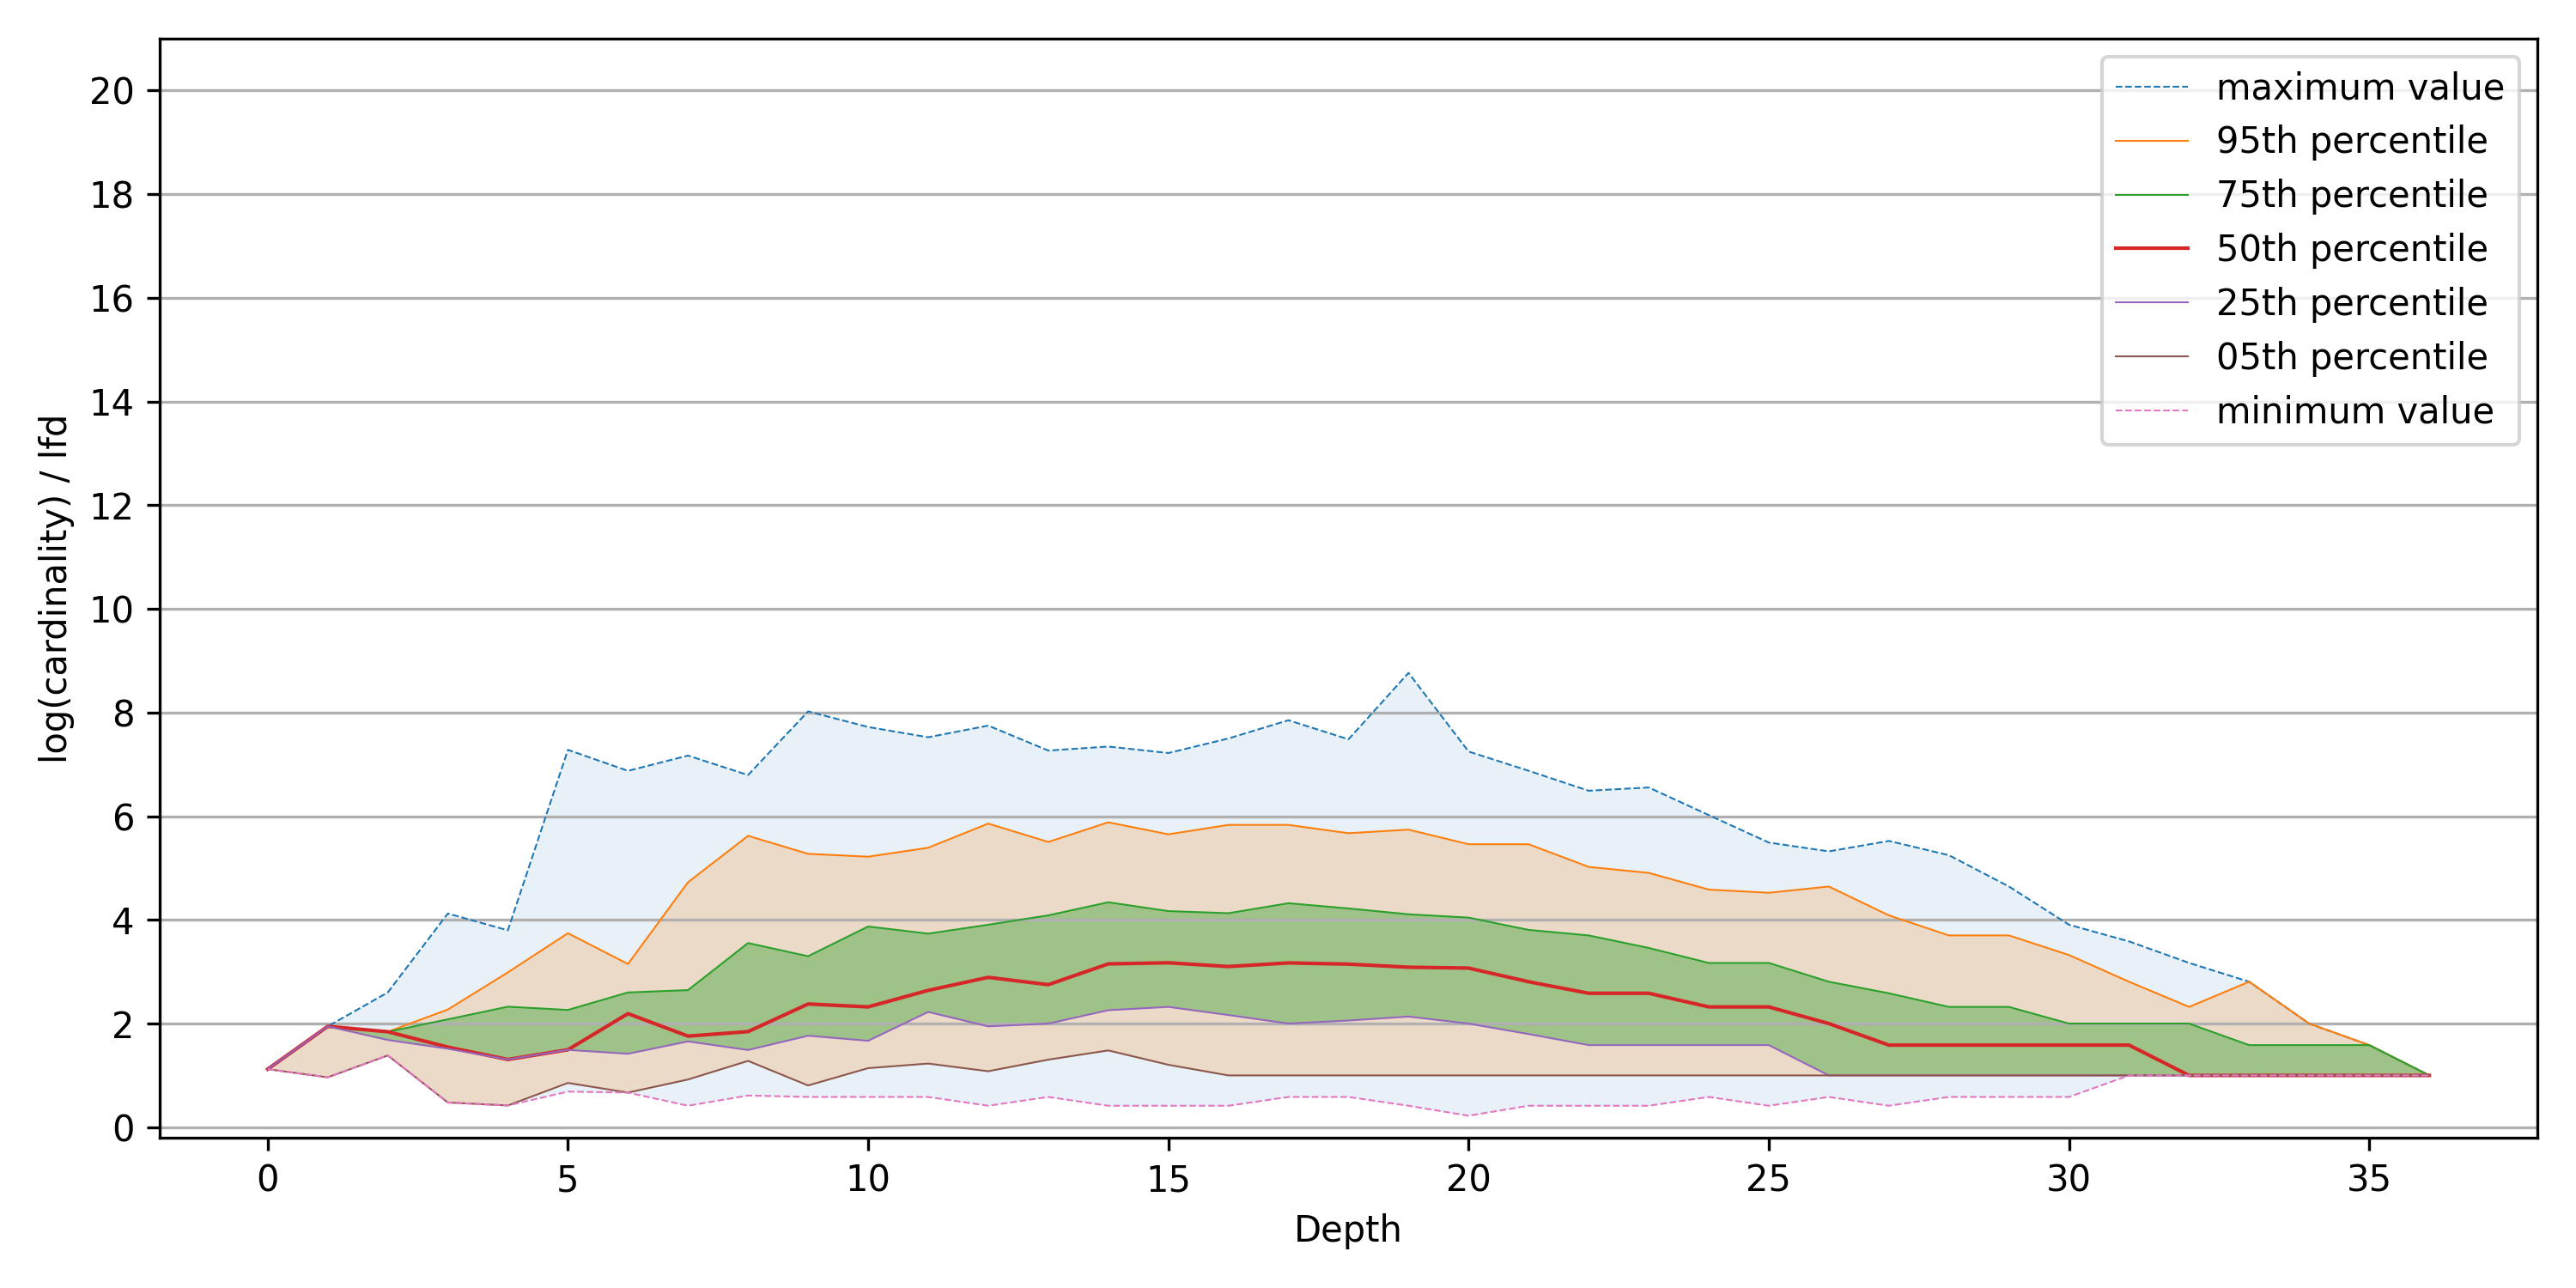
\includegraphics[width=0.95\textwidth]{images/lfd/fashion-mnist-60000.png}\\
        \subcaption{Fashion-mnist}
        \label{fig:results:fashion-mnist-lfd}
    \end{subfigure}%
    \begin{subfigure}[b]{0.47\textwidth}
        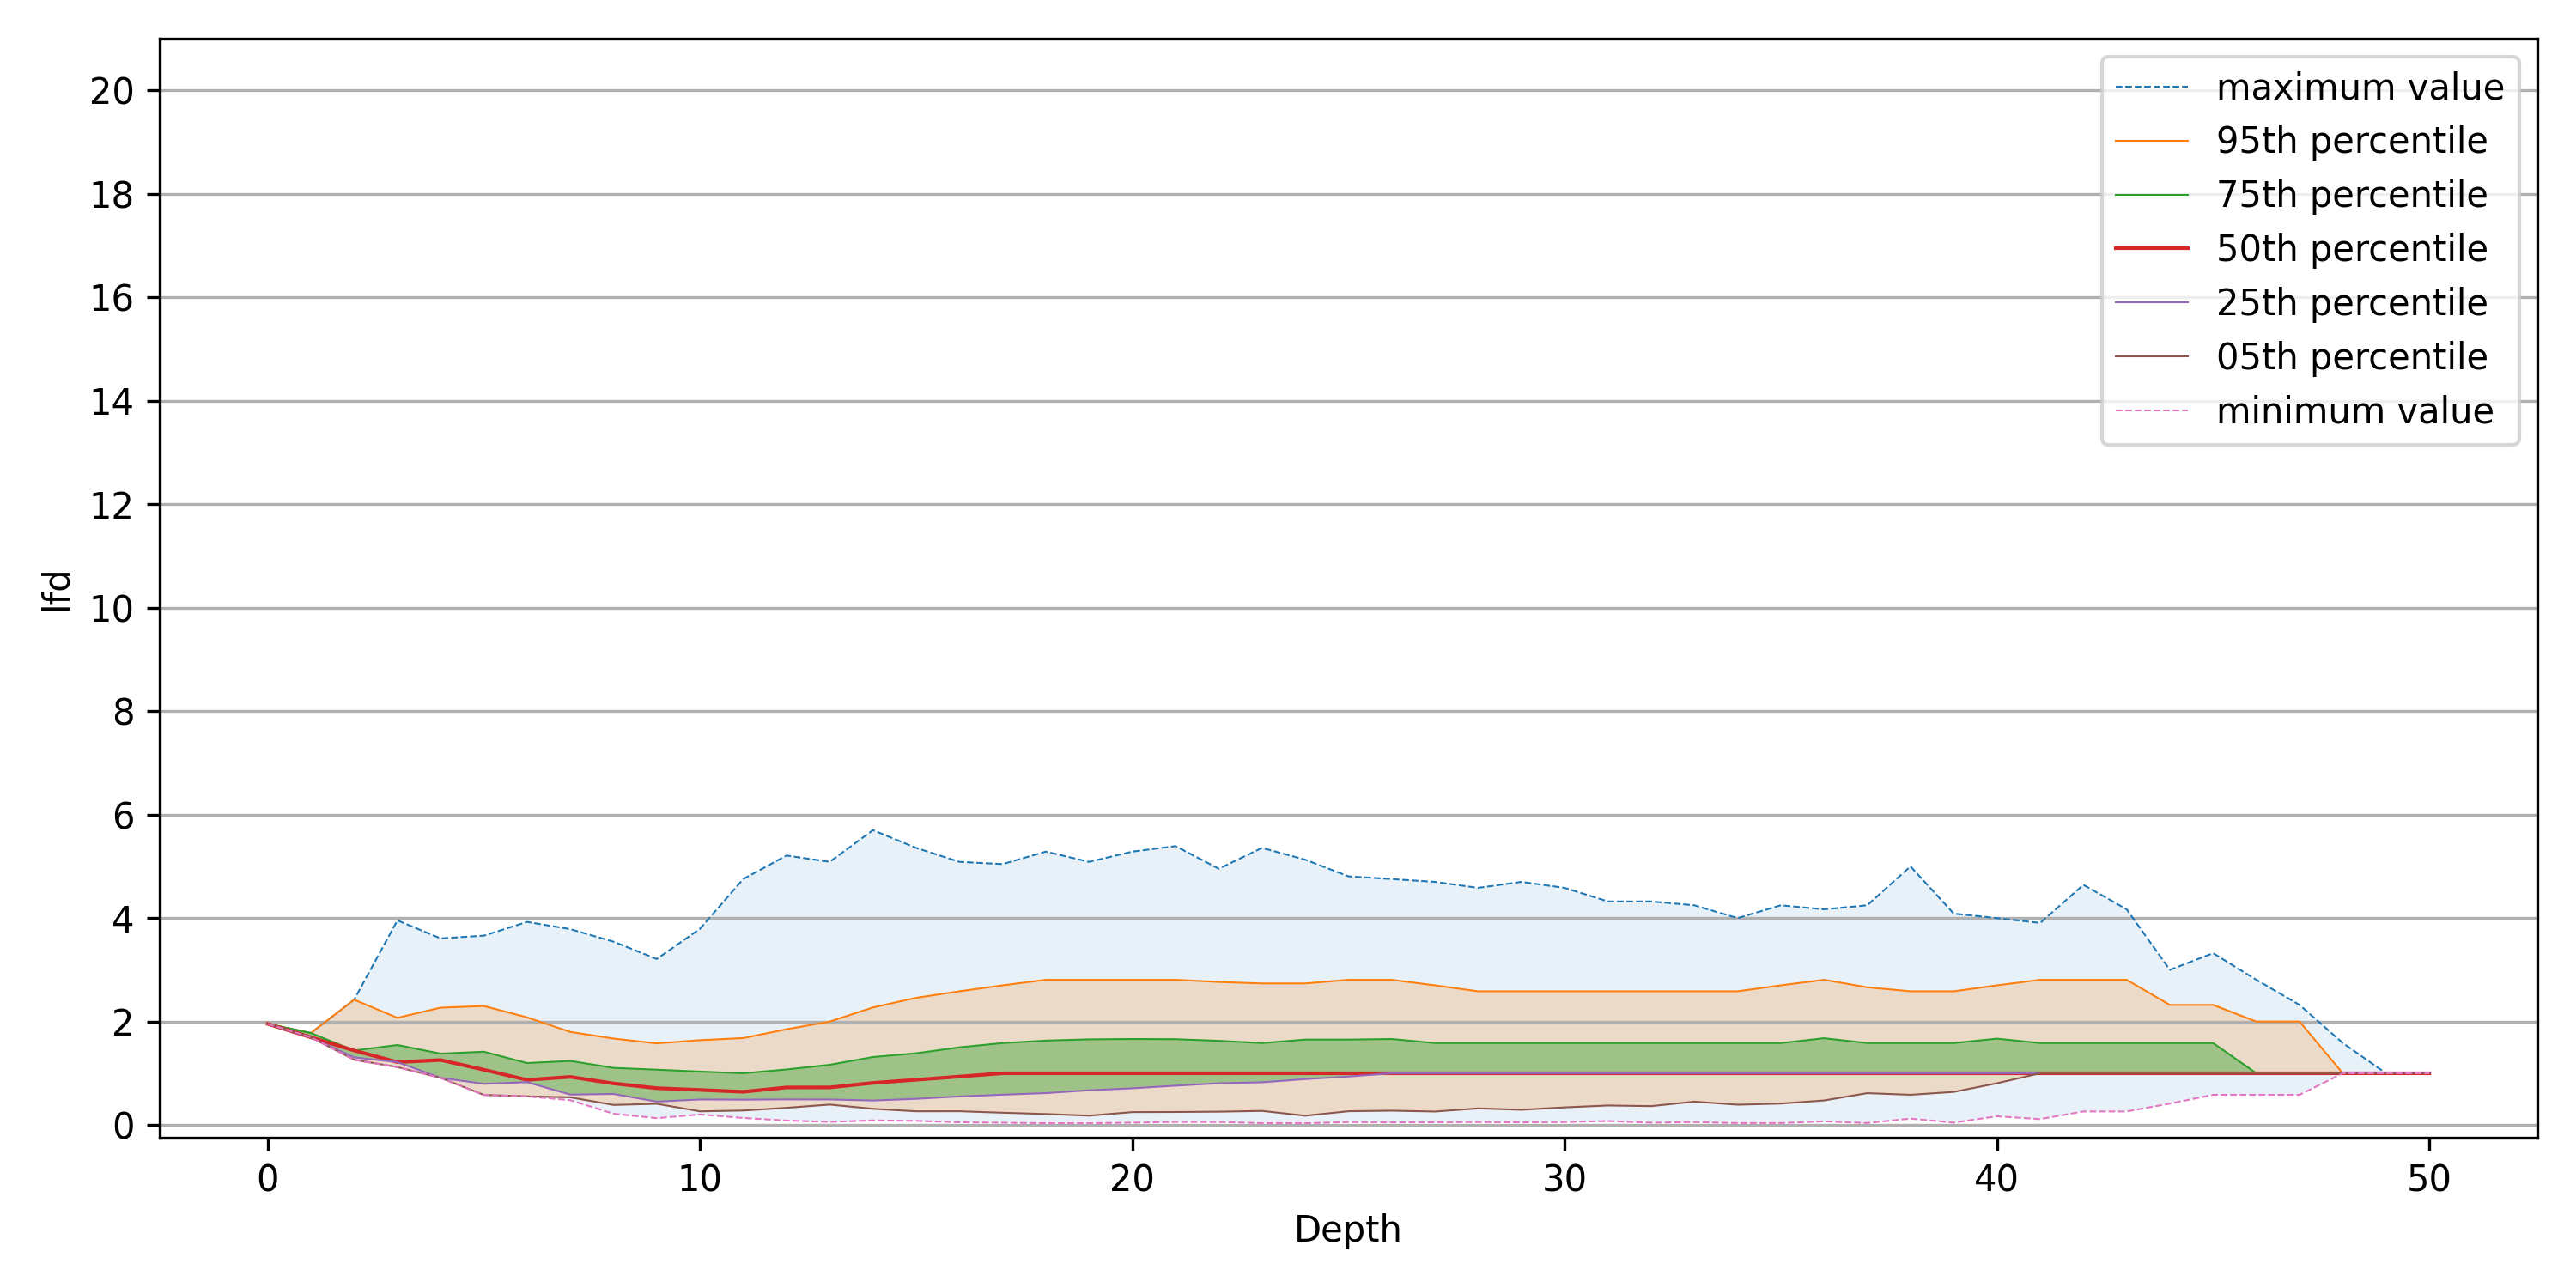
\includegraphics[width=0.95\textwidth]{images/lfd/glove-25-1183514.png}\\
        \subcaption{Glove-25}
        \label{fig:results:glove-25-lfd}
    \end{subfigure}
    \vspace{1em}
    \\
    \begin{subfigure}[b]{0.47\textwidth}
        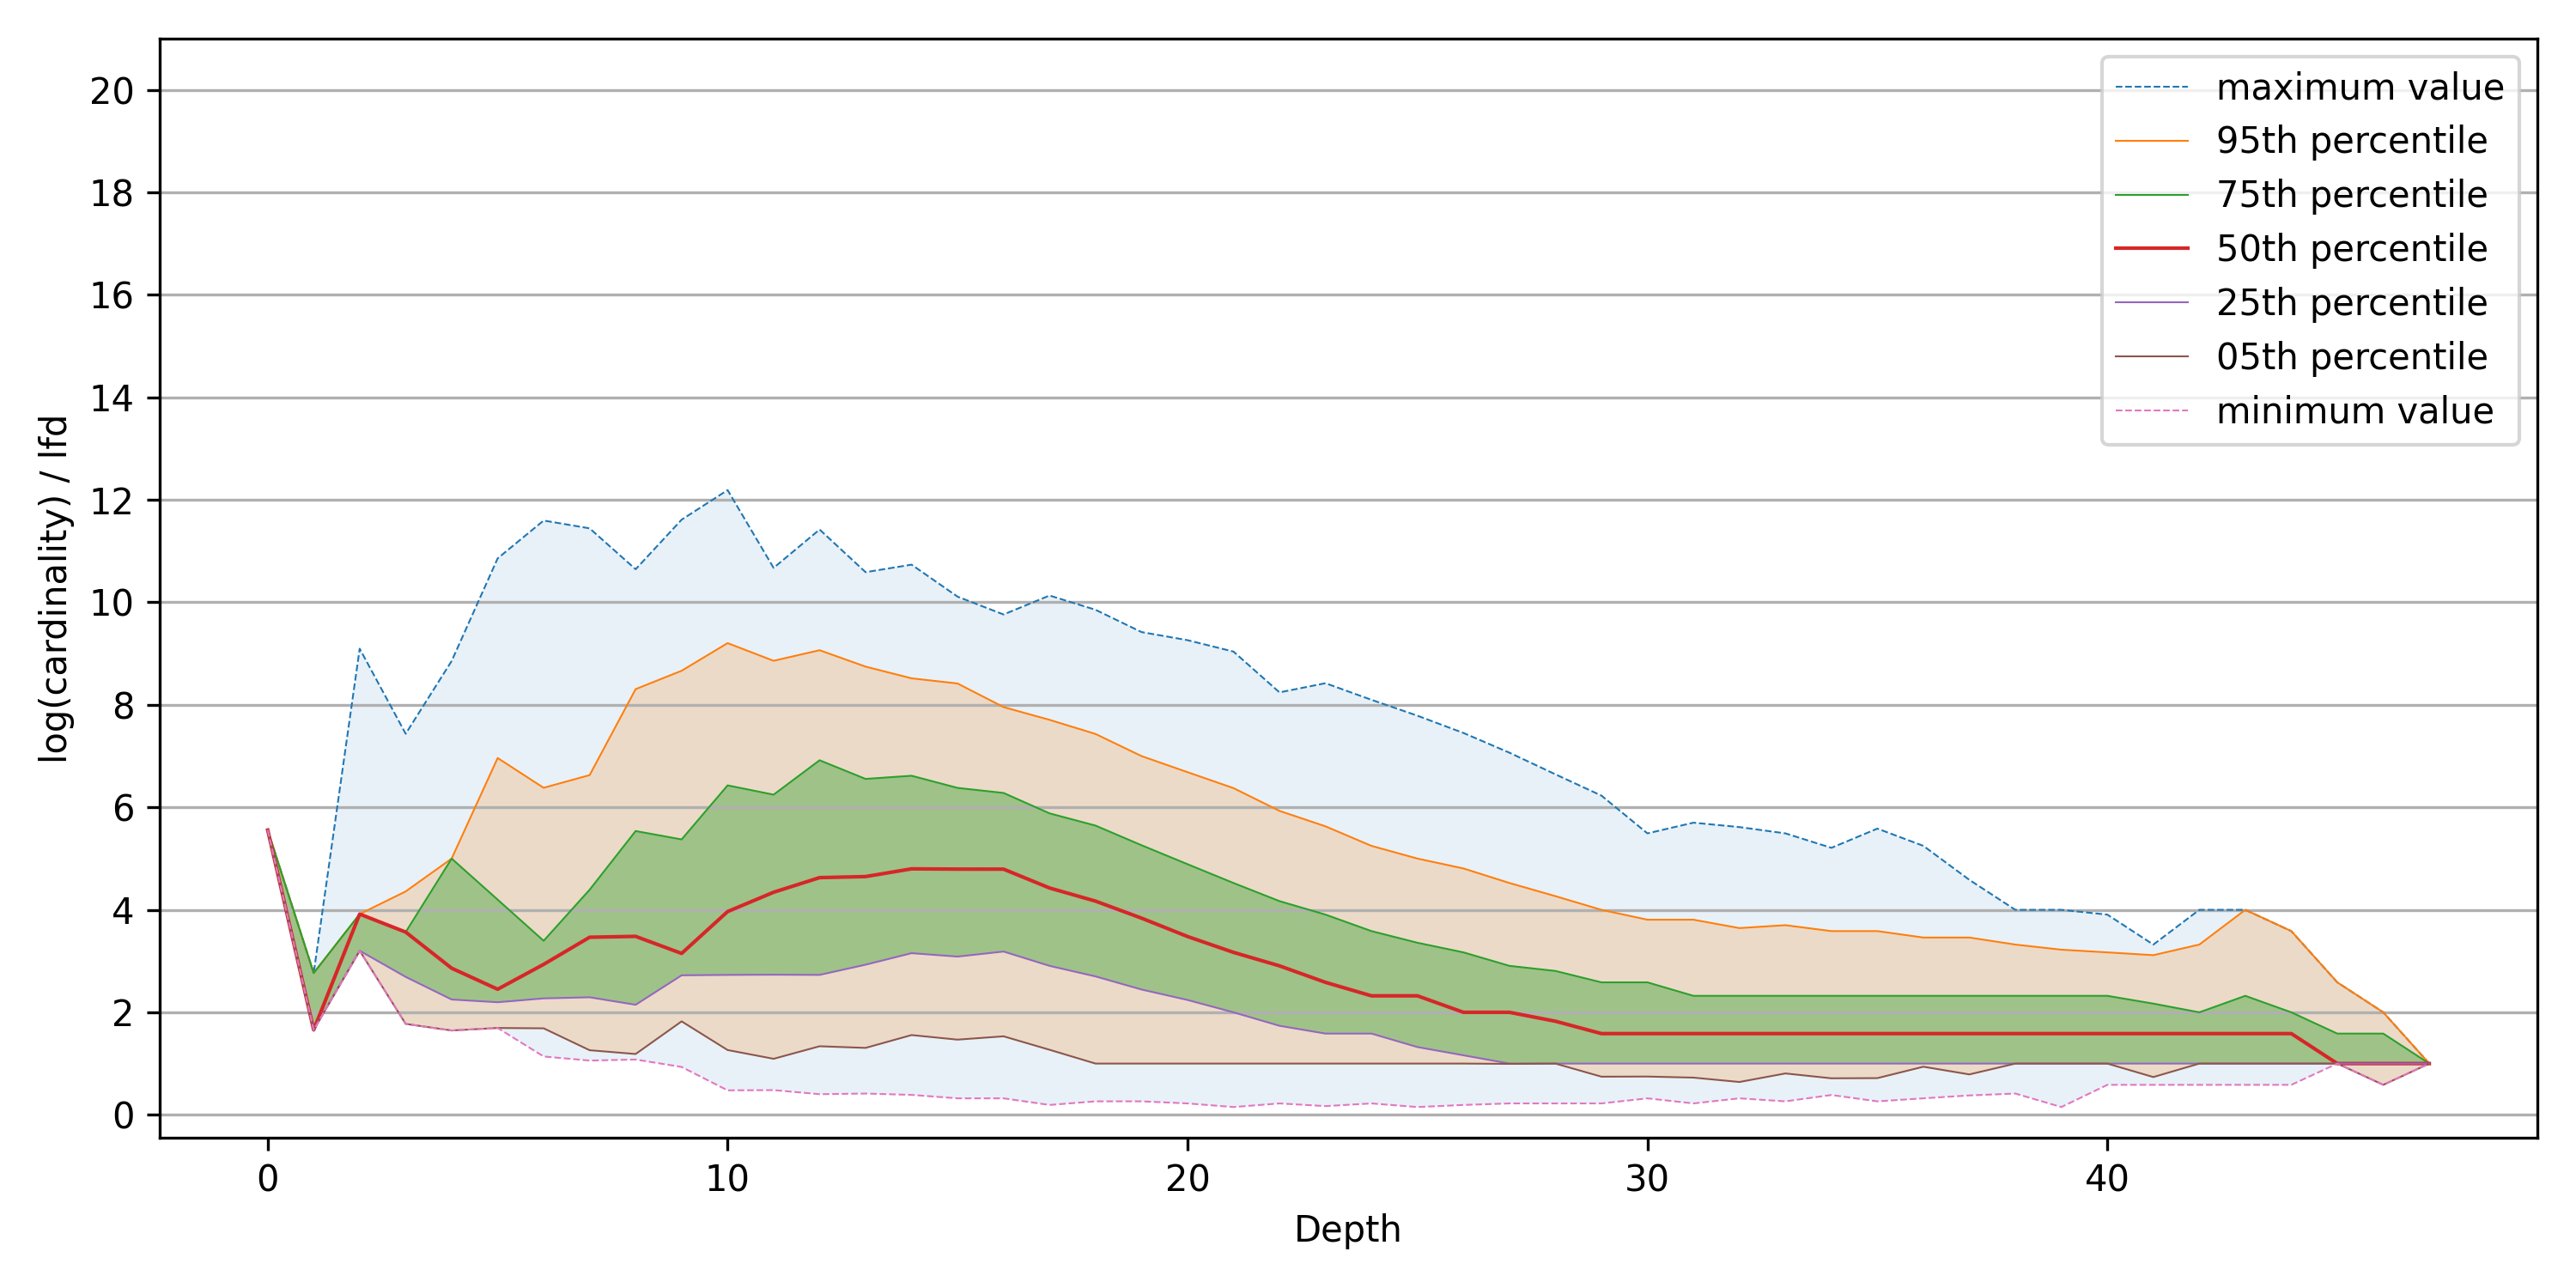
\includegraphics[width=0.95\textwidth]{images/lfd/sift-1000000.png}\\
        \subcaption{Sift}
        \label{fig:results:sift-lfd}
    \end{subfigure}%
    \begin{subfigure}[b]{0.47\textwidth}
        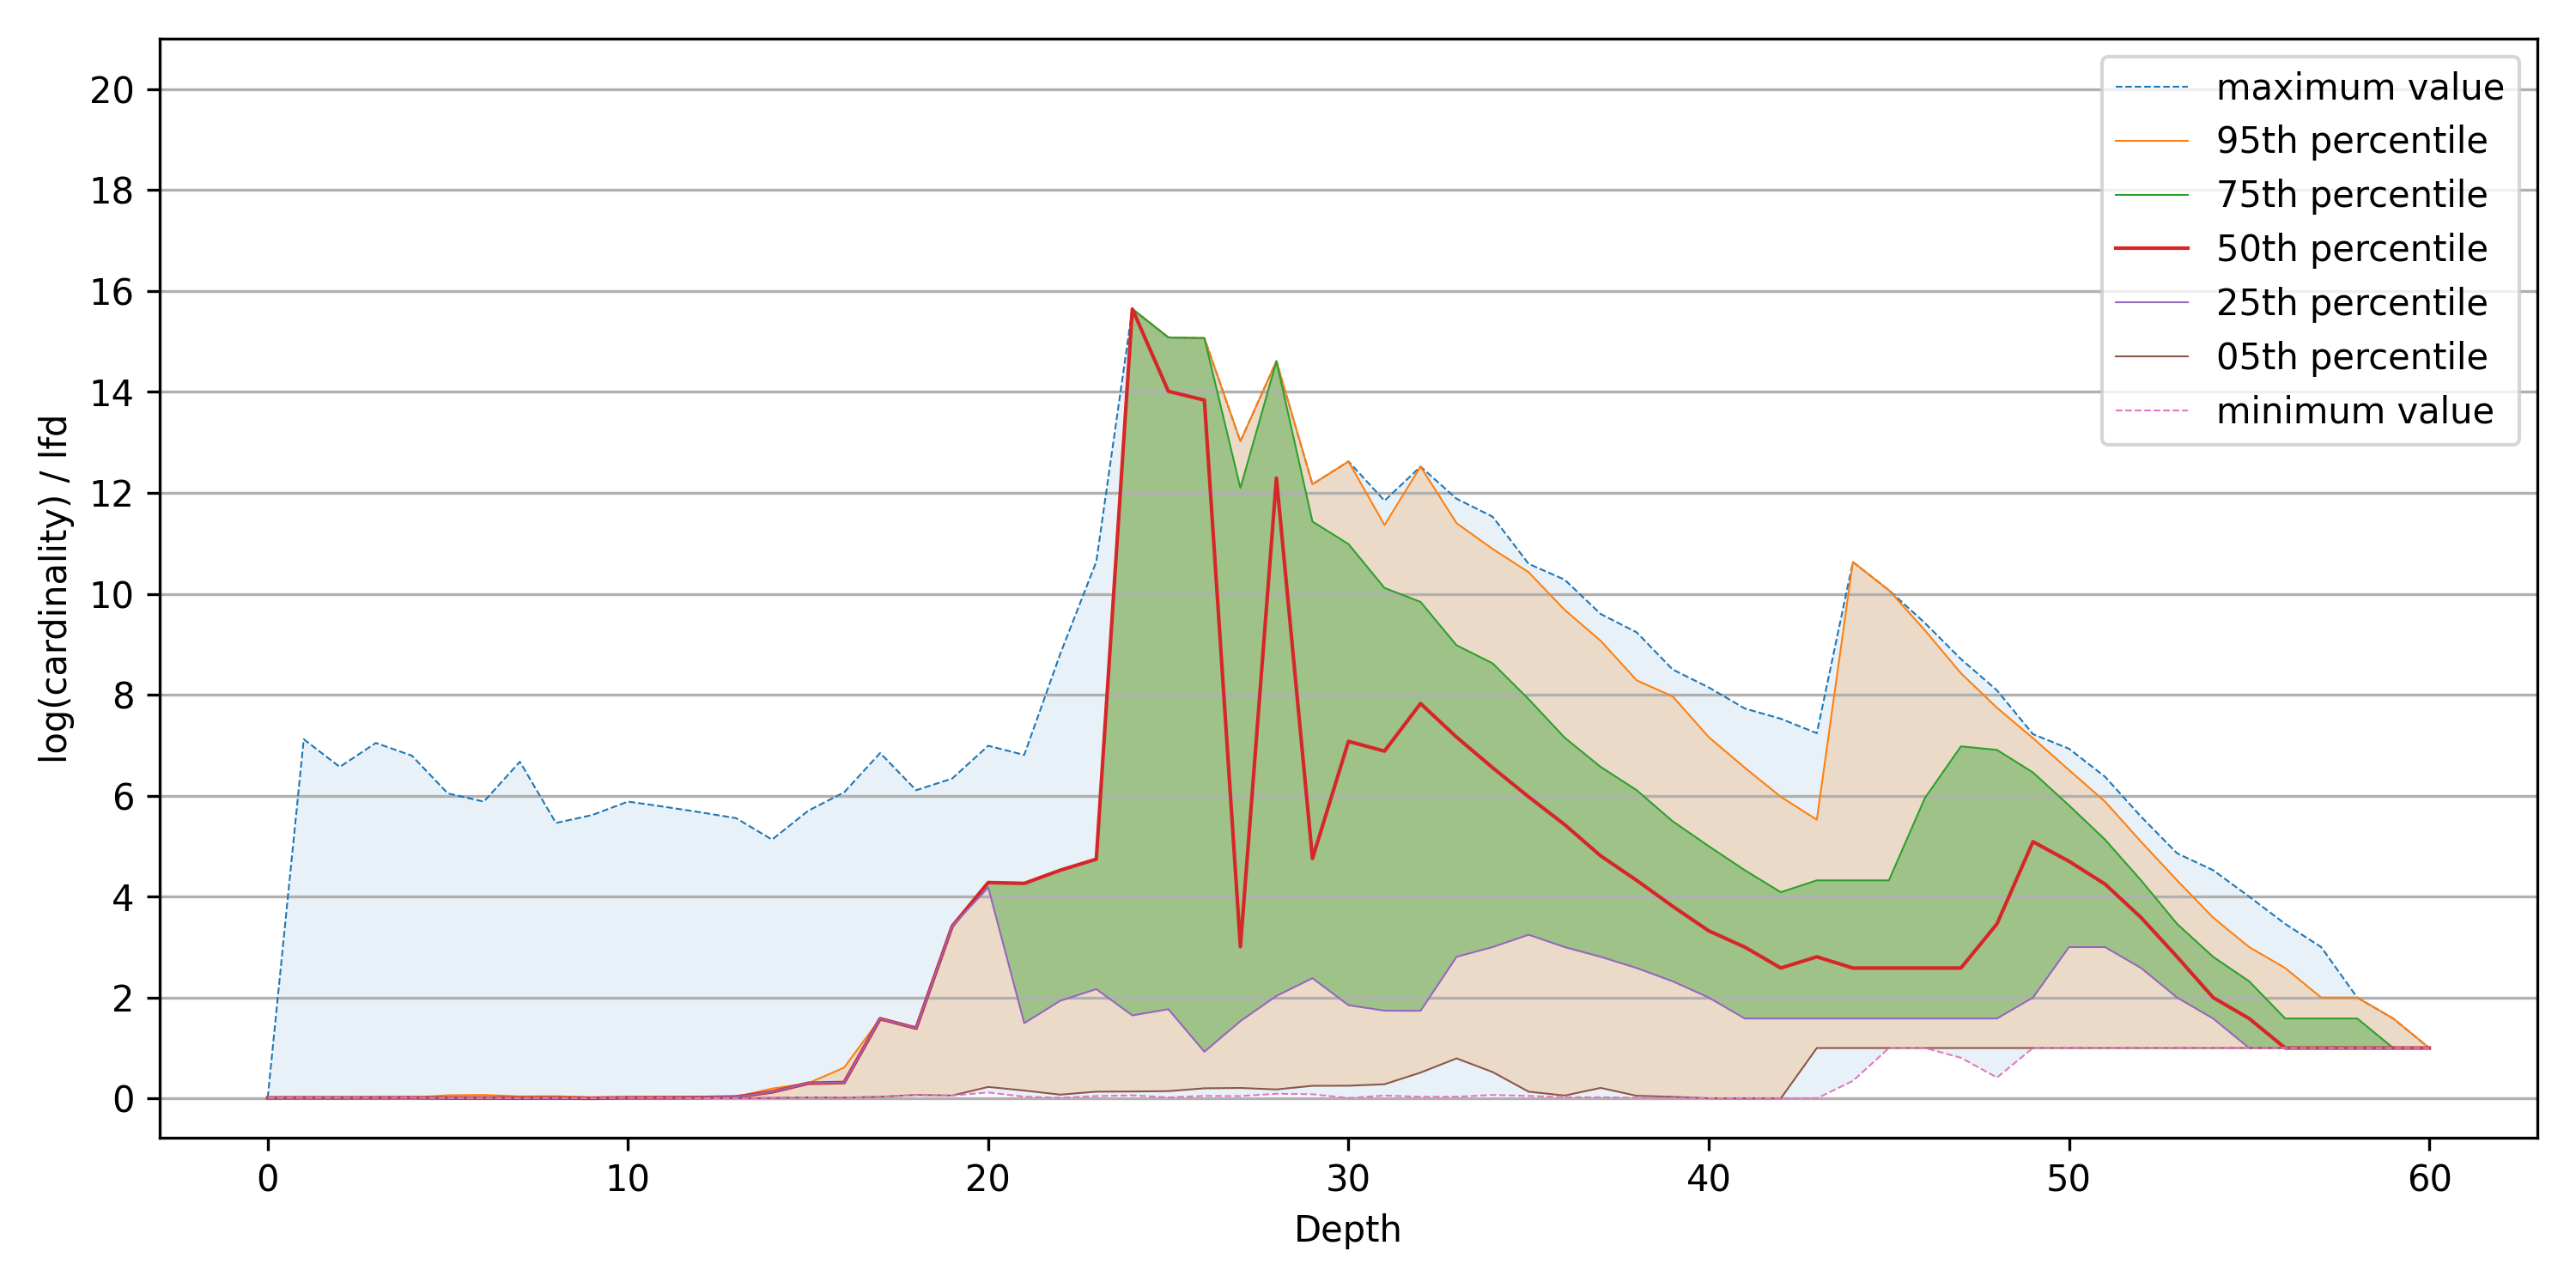
\includegraphics[width=0.95\textwidth]{images/lfd/radio-ml-97920.png}\\
        \subcaption{RadioML}
        \label{fig:results:radioml-lfd}
    \end{subfigure}%
    \\
    \begin{subfigure}[b]{0.47\textwidth}
        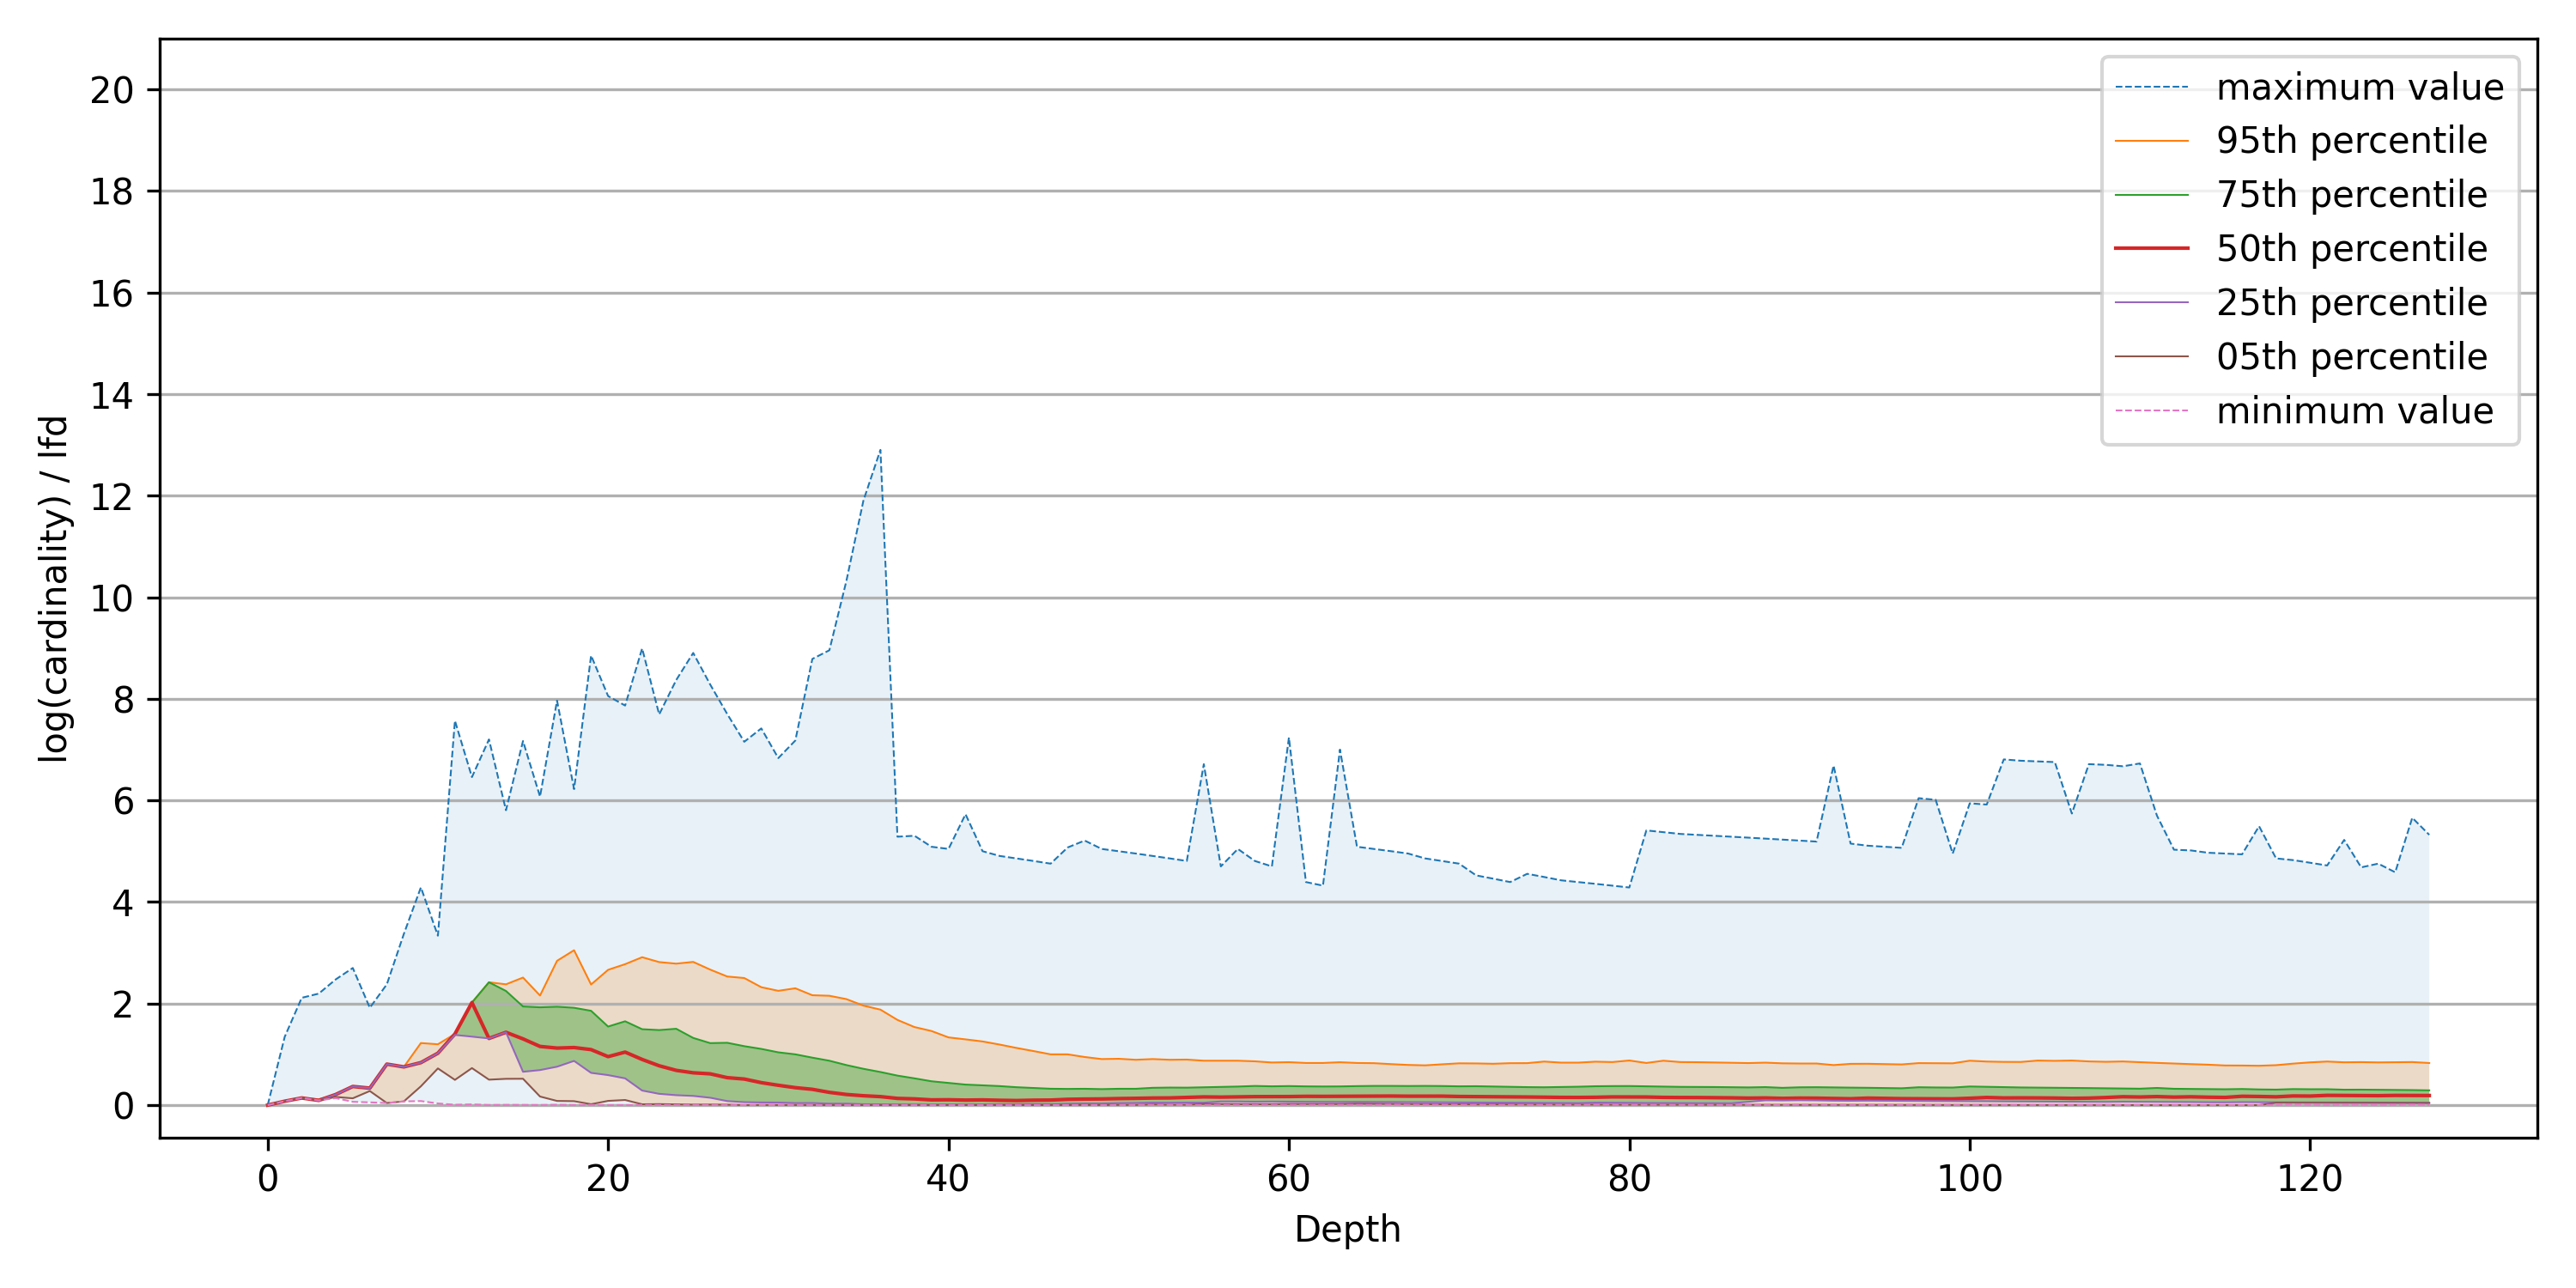
\includegraphics[width=0.95\textwidth]{images/lfd/silva-2224640.png}\\
        \subcaption{Silva 18S}
        \label{fig:results:silva-lfd}
    \end{subfigure}%  
    \begin{subfigure}[b]{0.47\textwidth}
        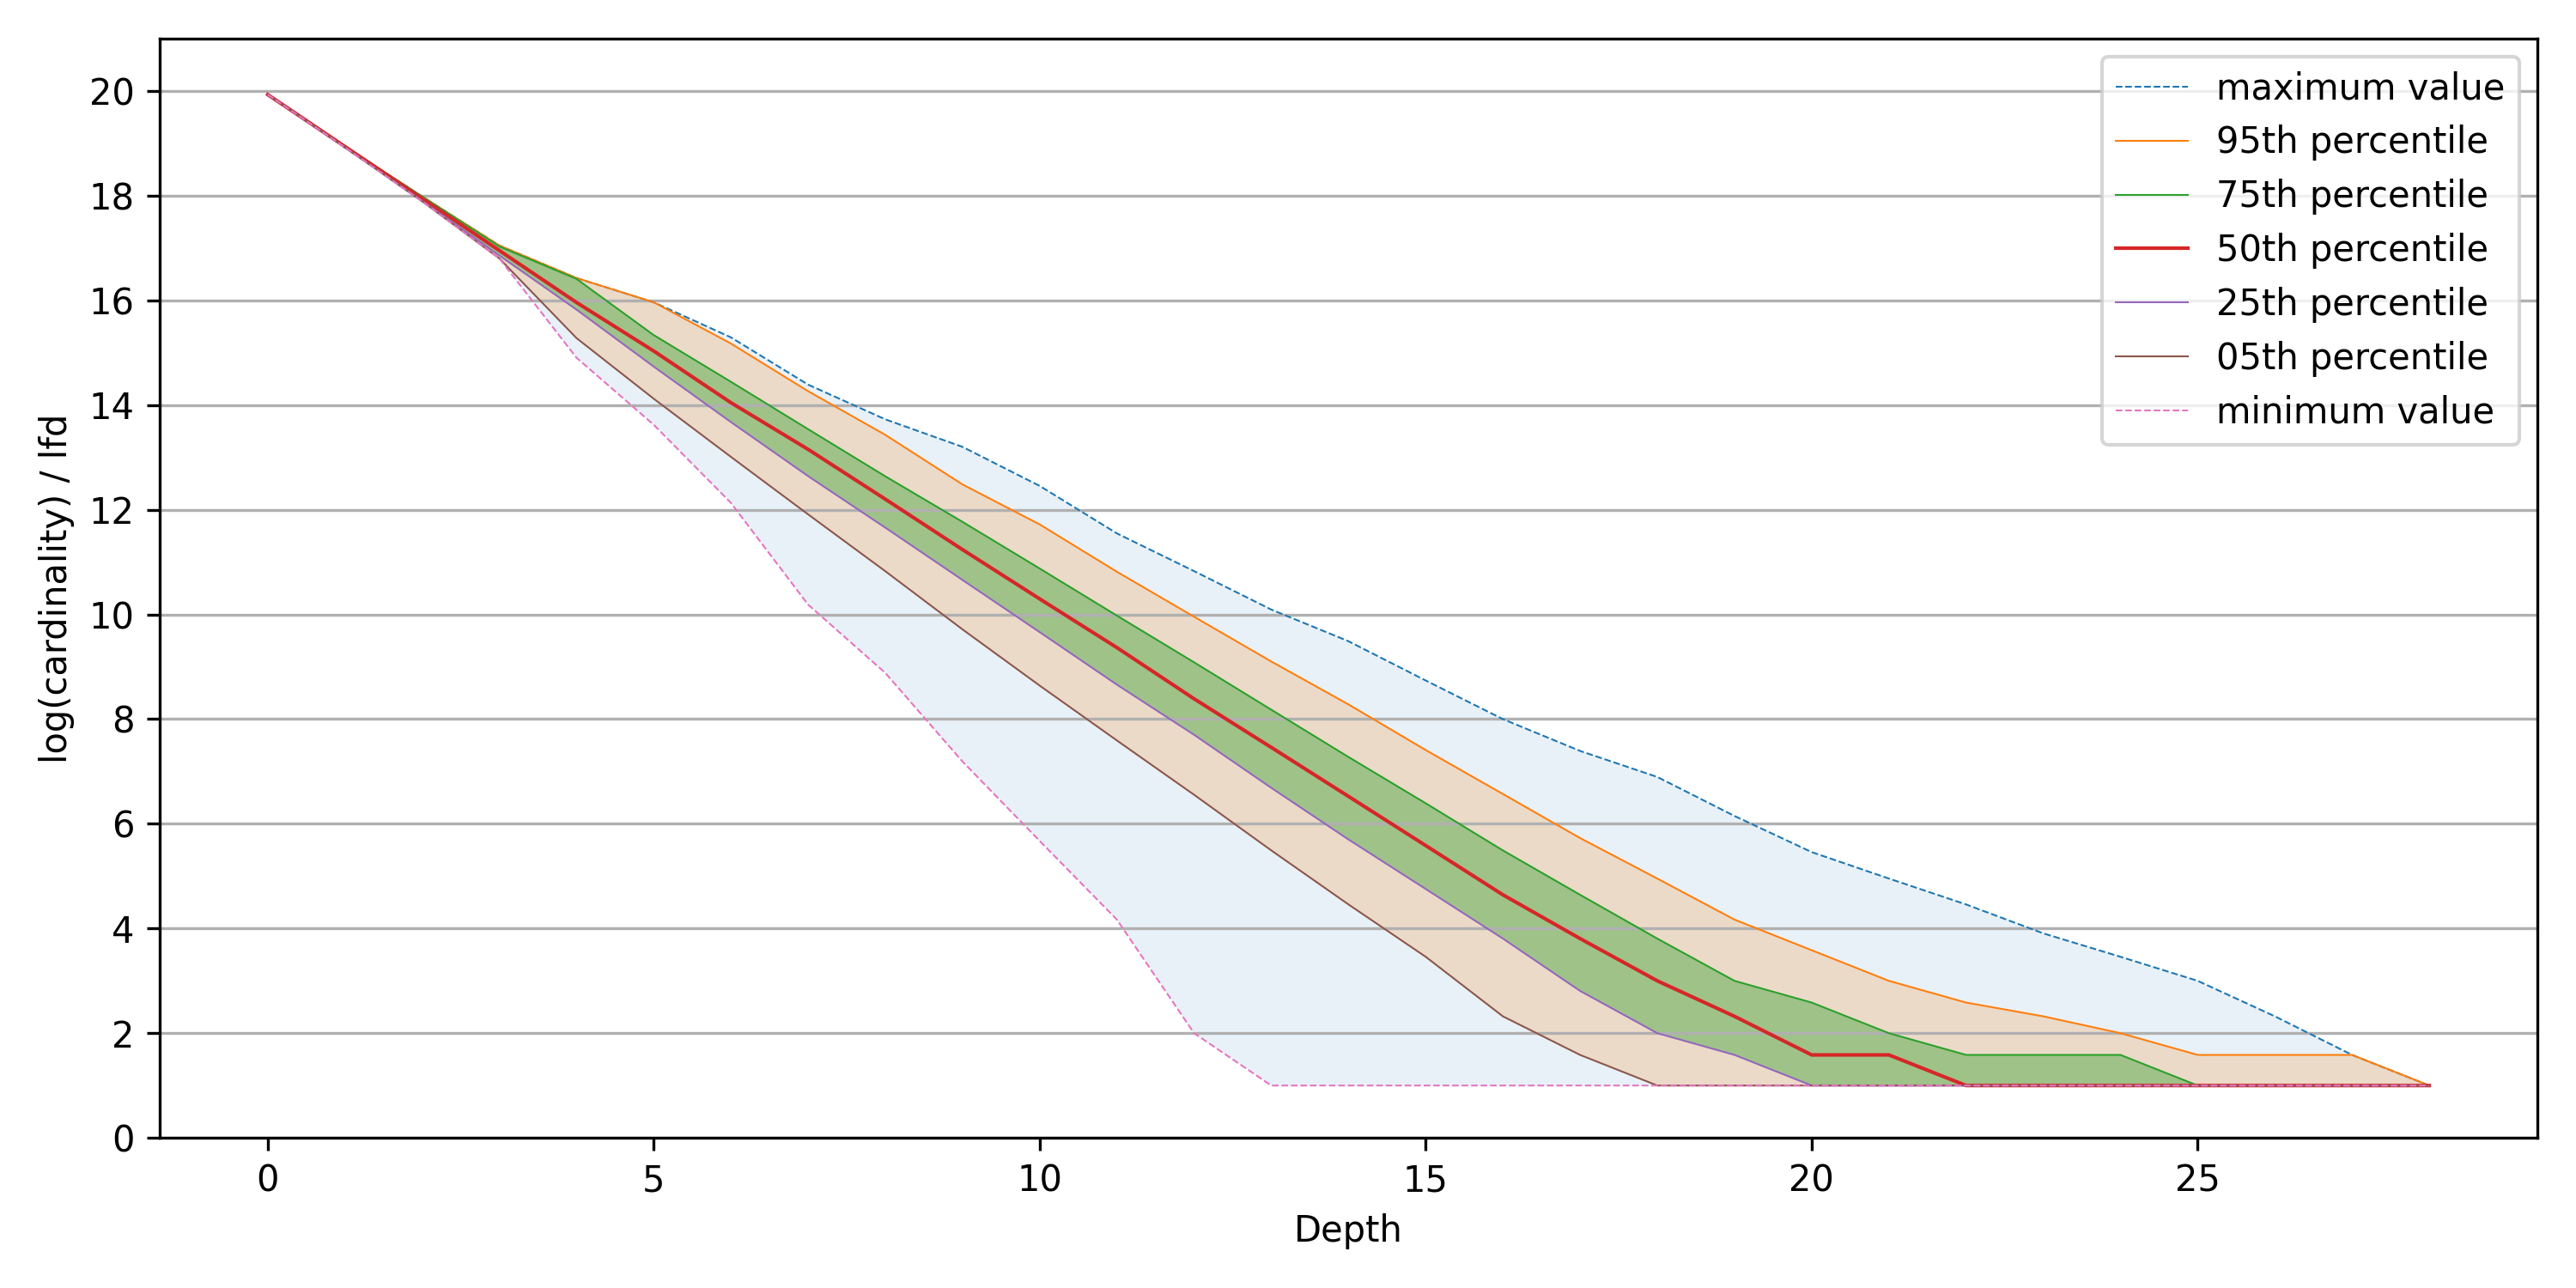
\includegraphics[width=0.95\textwidth]{images/lfd/random-1000000.png}\\
        \subcaption{A random dataset}
        \label{fig:results:random-lfd}
    \end{subfigure}
    \vspace{1em}
    \caption{Local fractal dimension vs. cluster depth across six datasets, grouped by decile of local fractal dimension and weighted by the cardinalities of the clusters.
    The last dataset is randomly generated.}
    \label{fig:results:lfd-plots}
\end{figure}


\subsection{Indexing and Tuning Time}
\label{sec:results:indexing-and-tuning-time}

For each of the ANN-benchmark datasets and the Random dataset, we report the time taken for each algorithm to build the index and to tune the hyper-parameters for these indices to achieve the highest possible recall.
Though CAKES has three different algorithms, they share the same tree and so they have the same indexing time.
Thus, we show CAKES's indexing time only once.

The plots in Figure~\ref{fig:results:indexing} show the results of these benchmarks.
The horizontal axis in each subplot shows the cardinality of the dataset augmented with synthetic points (see Section \ref{sec:methods:synthetic-data}).
The left-most point on each line is at the cardinality of the original dataset without any synthetic augmentation.
The vertical axis denotes the sum of indexing and tuning time in seconds.
Both axes are on a logarithmic scale.
Hereafter, when we refer to the ``indexing time'' of an algorithm, we are implicitly referring to the sum of indexing and tuning time for said algorithm.

{\color{red} TODO: remove all red TODOs.}

{\color{red} TODO: Add more red TODOs.}

{\color{red} TODO: Figure out if we should remove all red TODOs or add more red TODOS}

On all datasets, we observe that the indexing time for CAKES increases roughly linearly as cardinality increases.
HNSW and ANNOY have the slowest indexing times across all the algorithms we benchmarked for each of the four datasets, at each cardinality. 
On some datasets, HNSW and ANNOY exhibit indexing times which are orders of magnitude slower than that of CAKES.
FAISS-Flat also exhibits the fastest indexing time on each dataset. 
This is not surprising, given that FAISS-Flat is a naive linear search algorithm and is not building an index.

We also highlight some differences in indexing time between different datasets.
With Fashion-Mnist, as shown in Figure~\ref{fig:results:fashion-mnist-indexing}, we observe that the indexing time for CAKES is lower than that of FAISS-IVF for all cardinalities.
With Glove-25 (see Figure~\ref{fig:results:glove-25-indexing}), however, at cardinalities greater than $10^7$, FAISS-IVF has lower indexing time than CAKES.
With Sift, CAKEs's indexing time is faster than that of FAISS-IVF until a cardinality of nearly $10^8$, and with the Random dataset, we observe that CAKES has faster indexing time than FAISS-IVF until a cardinality of nearly $10^7$.


\begin{figure}
    \begin{subfigure}[b]{0.47\textwidth}
        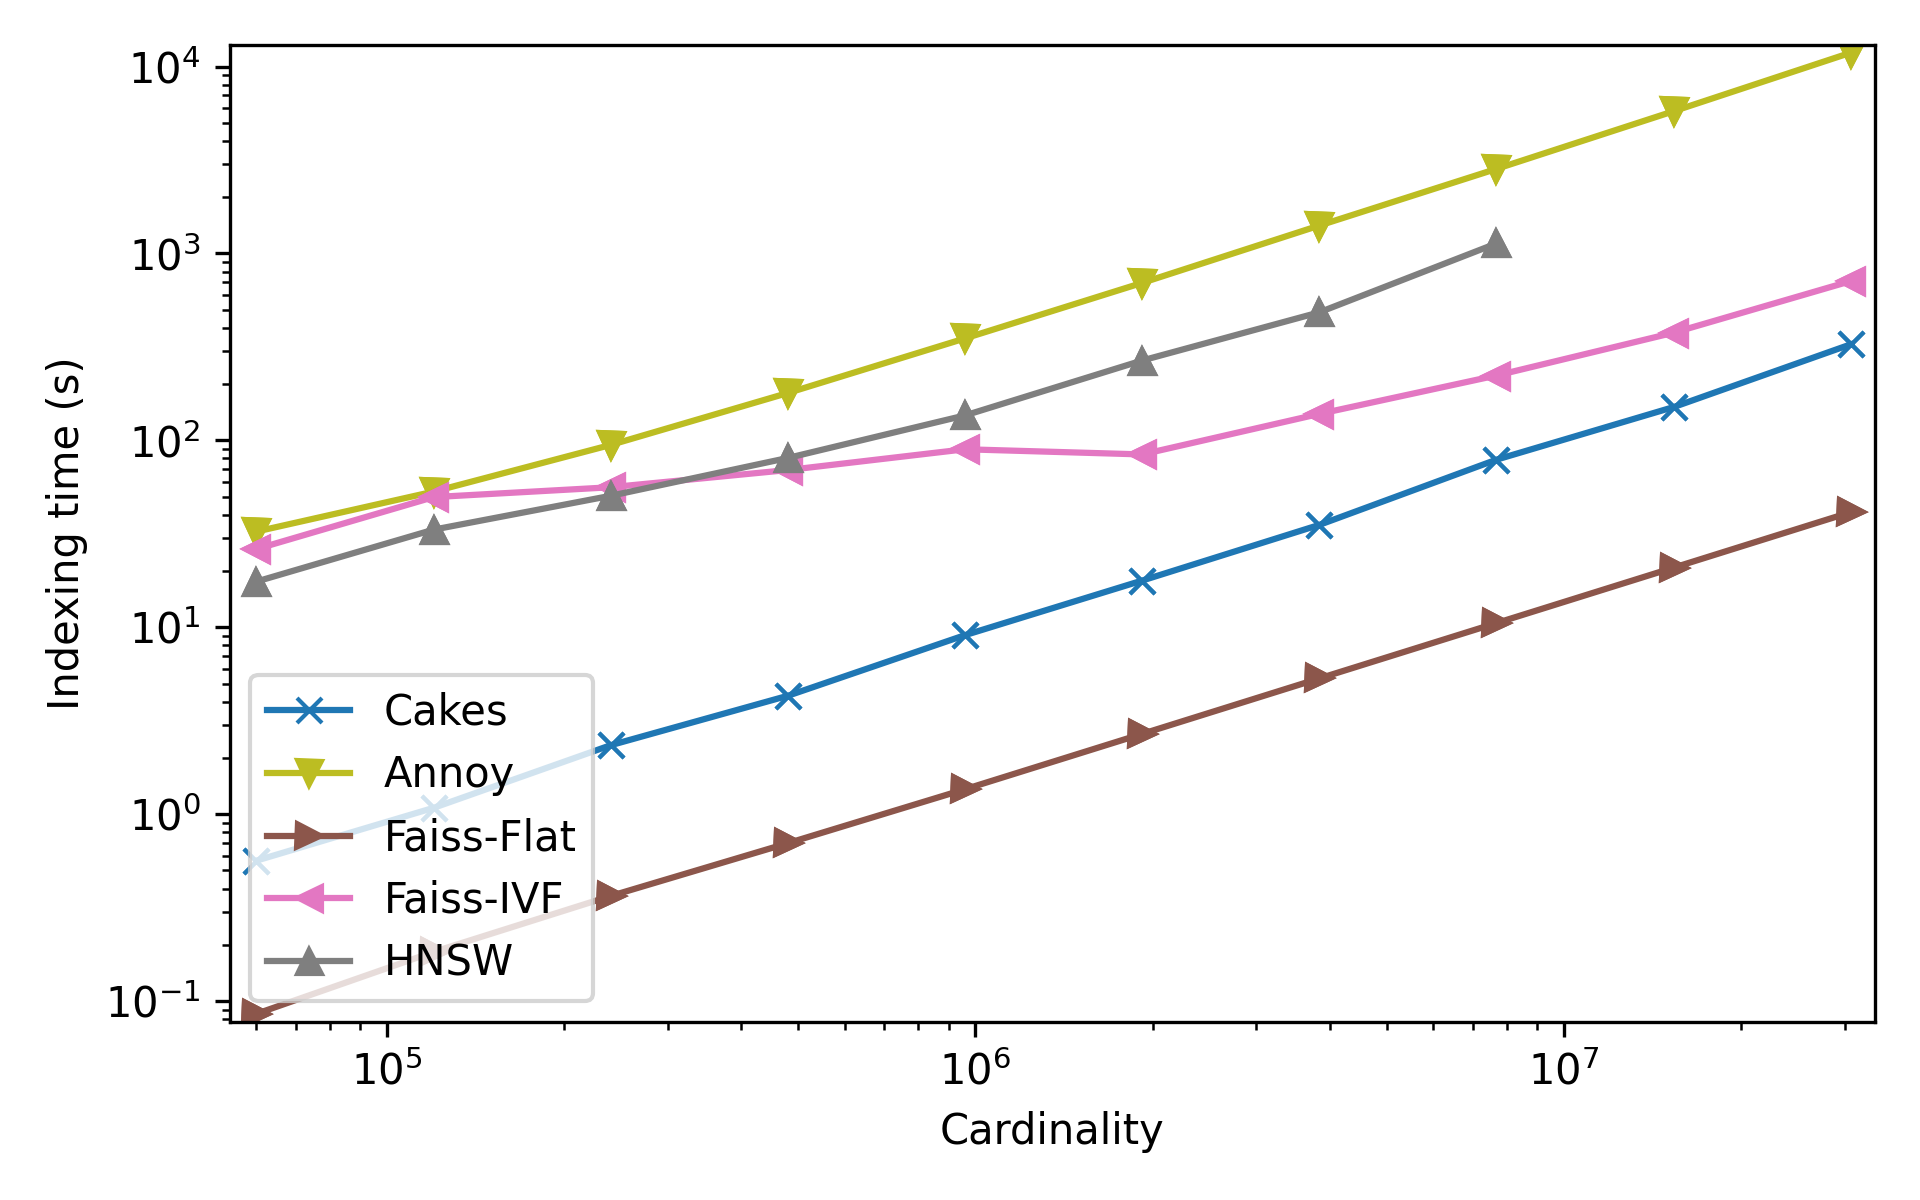
\includegraphics[width=0.95\textwidth]{plots/fashion-mnist-indexing.png}\\
        \subcaption{Fashion-mnist}
        \label{fig:results:fashion-mnist-indexing}
    \end{subfigure}%
    \begin{subfigure}[b]{0.47\textwidth}
        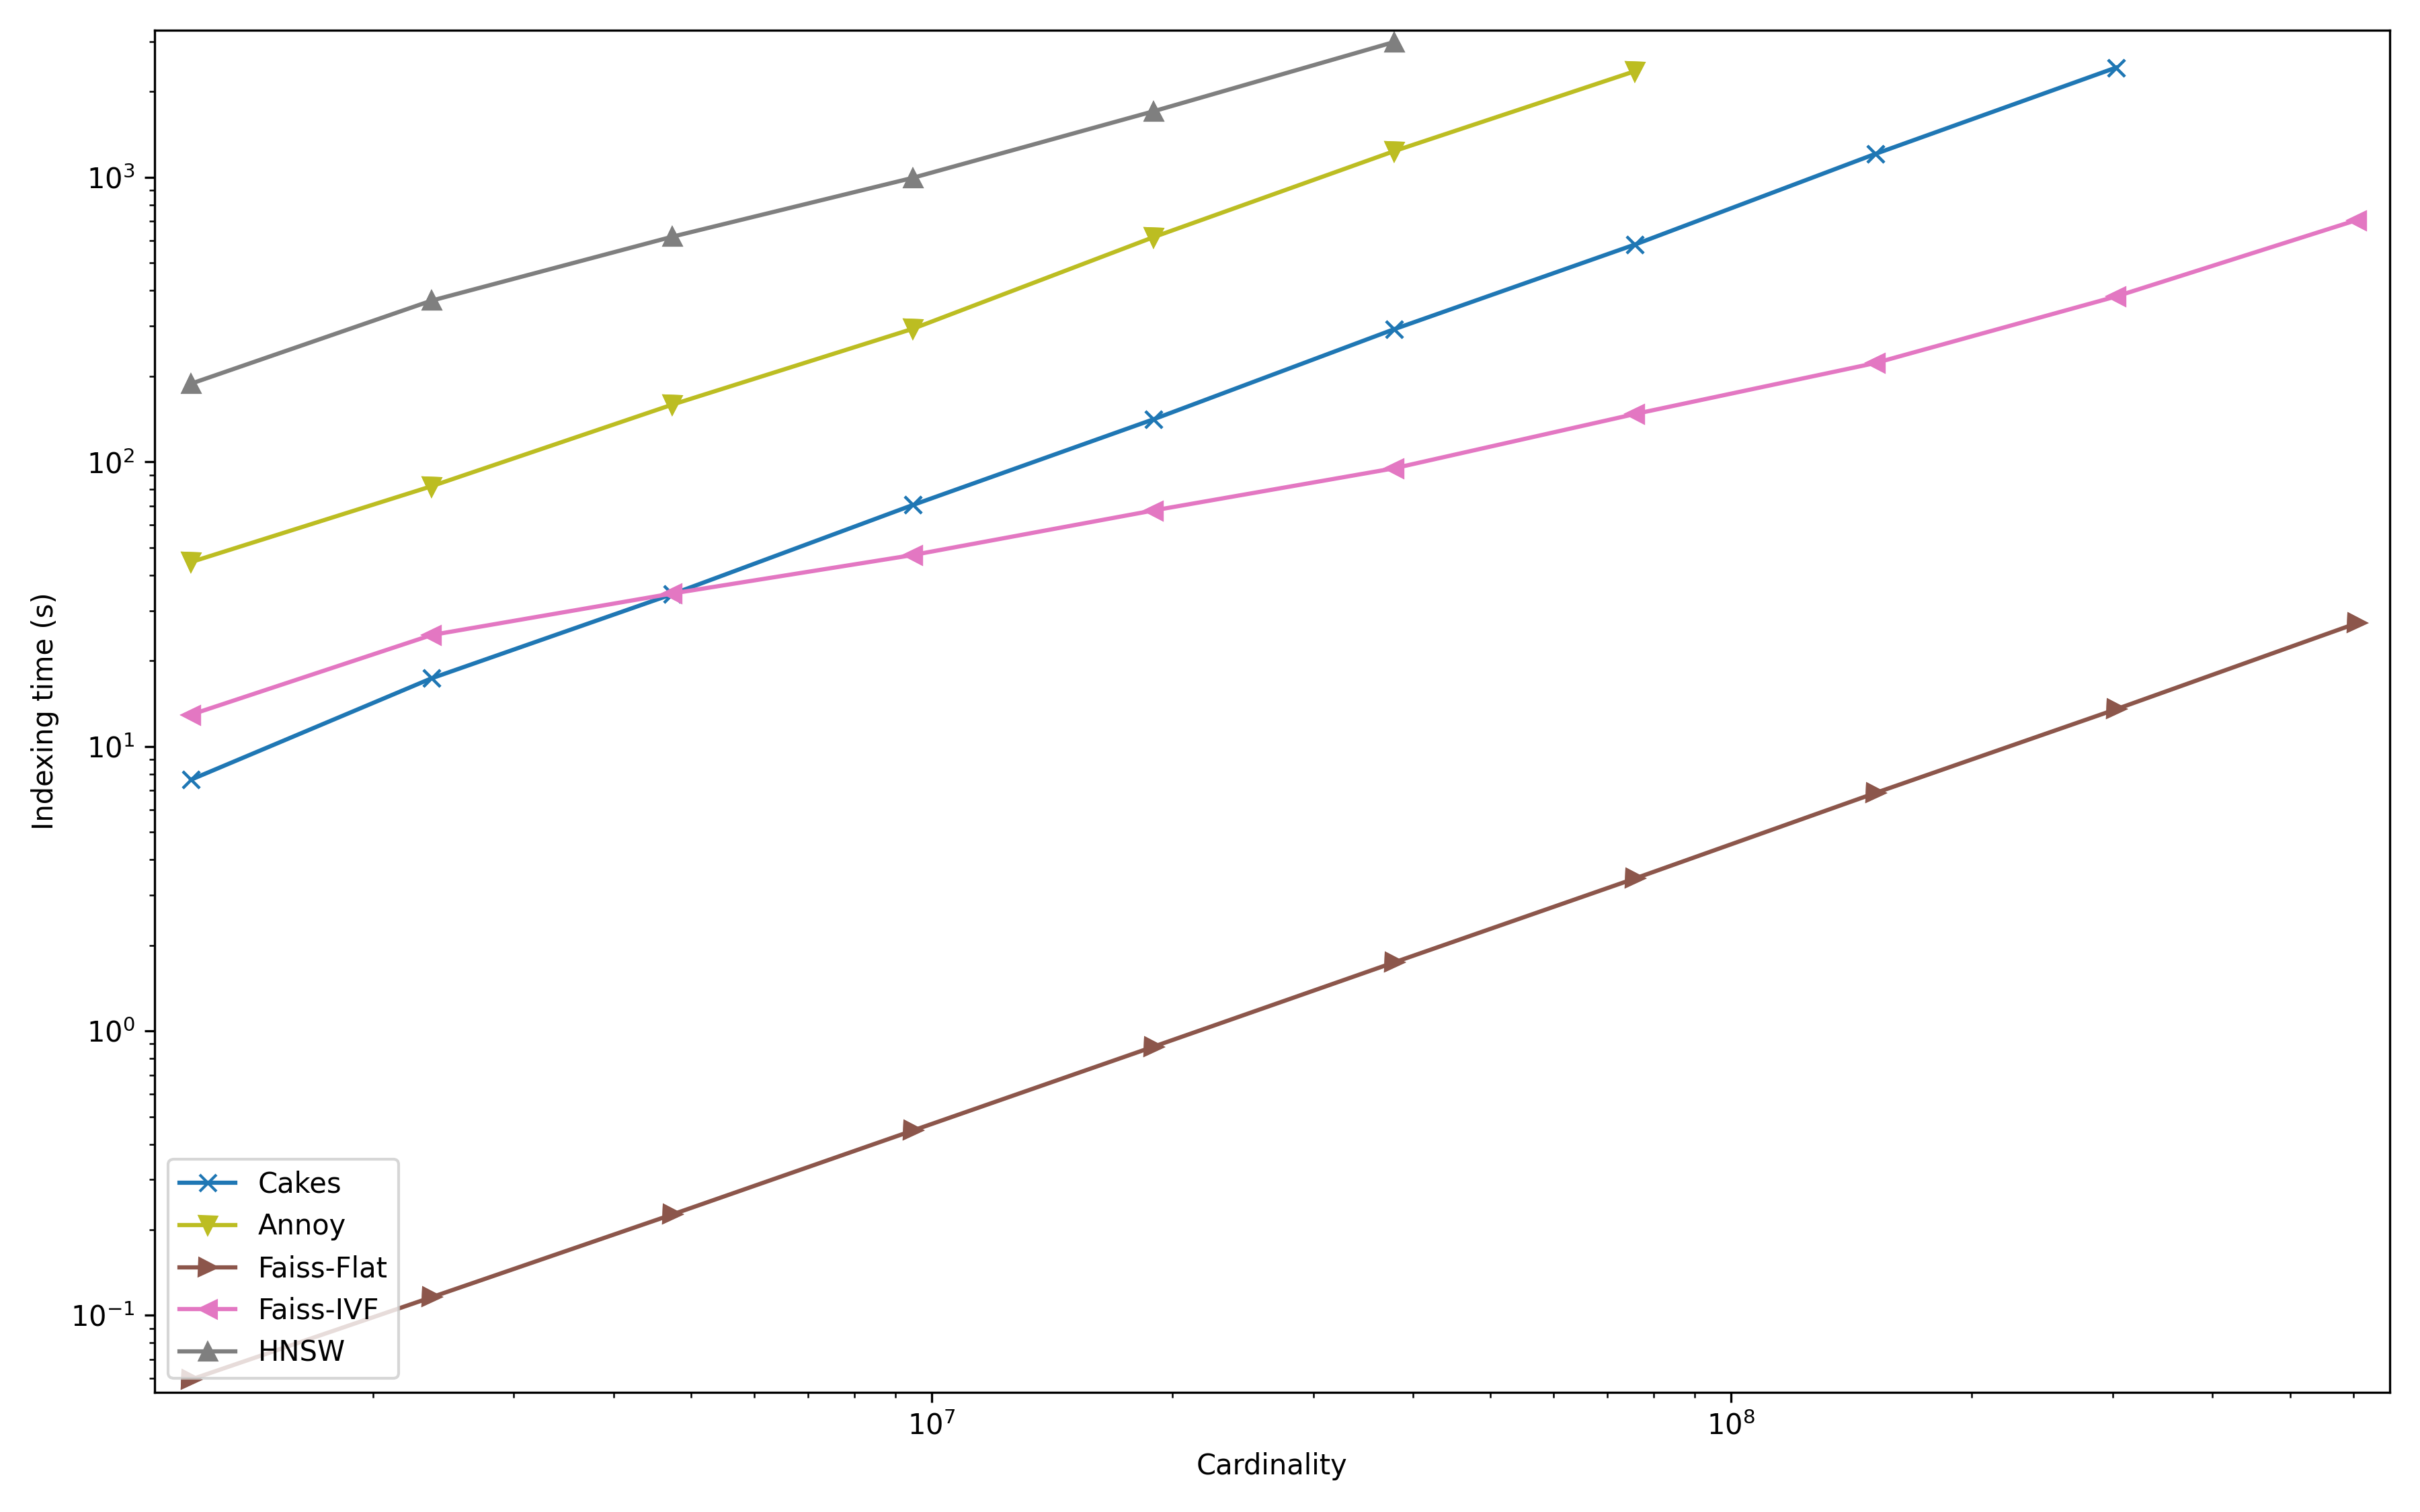
\includegraphics[width=0.95\textwidth]{plots/glove-25-indexing.png}\\
        \subcaption{Glove-25}
        \label{fig:results:glove-25-indexing}
    \end{subfigure}
    \vspace{1em}
    \\
    \begin{subfigure}[b]{0.47\textwidth}
        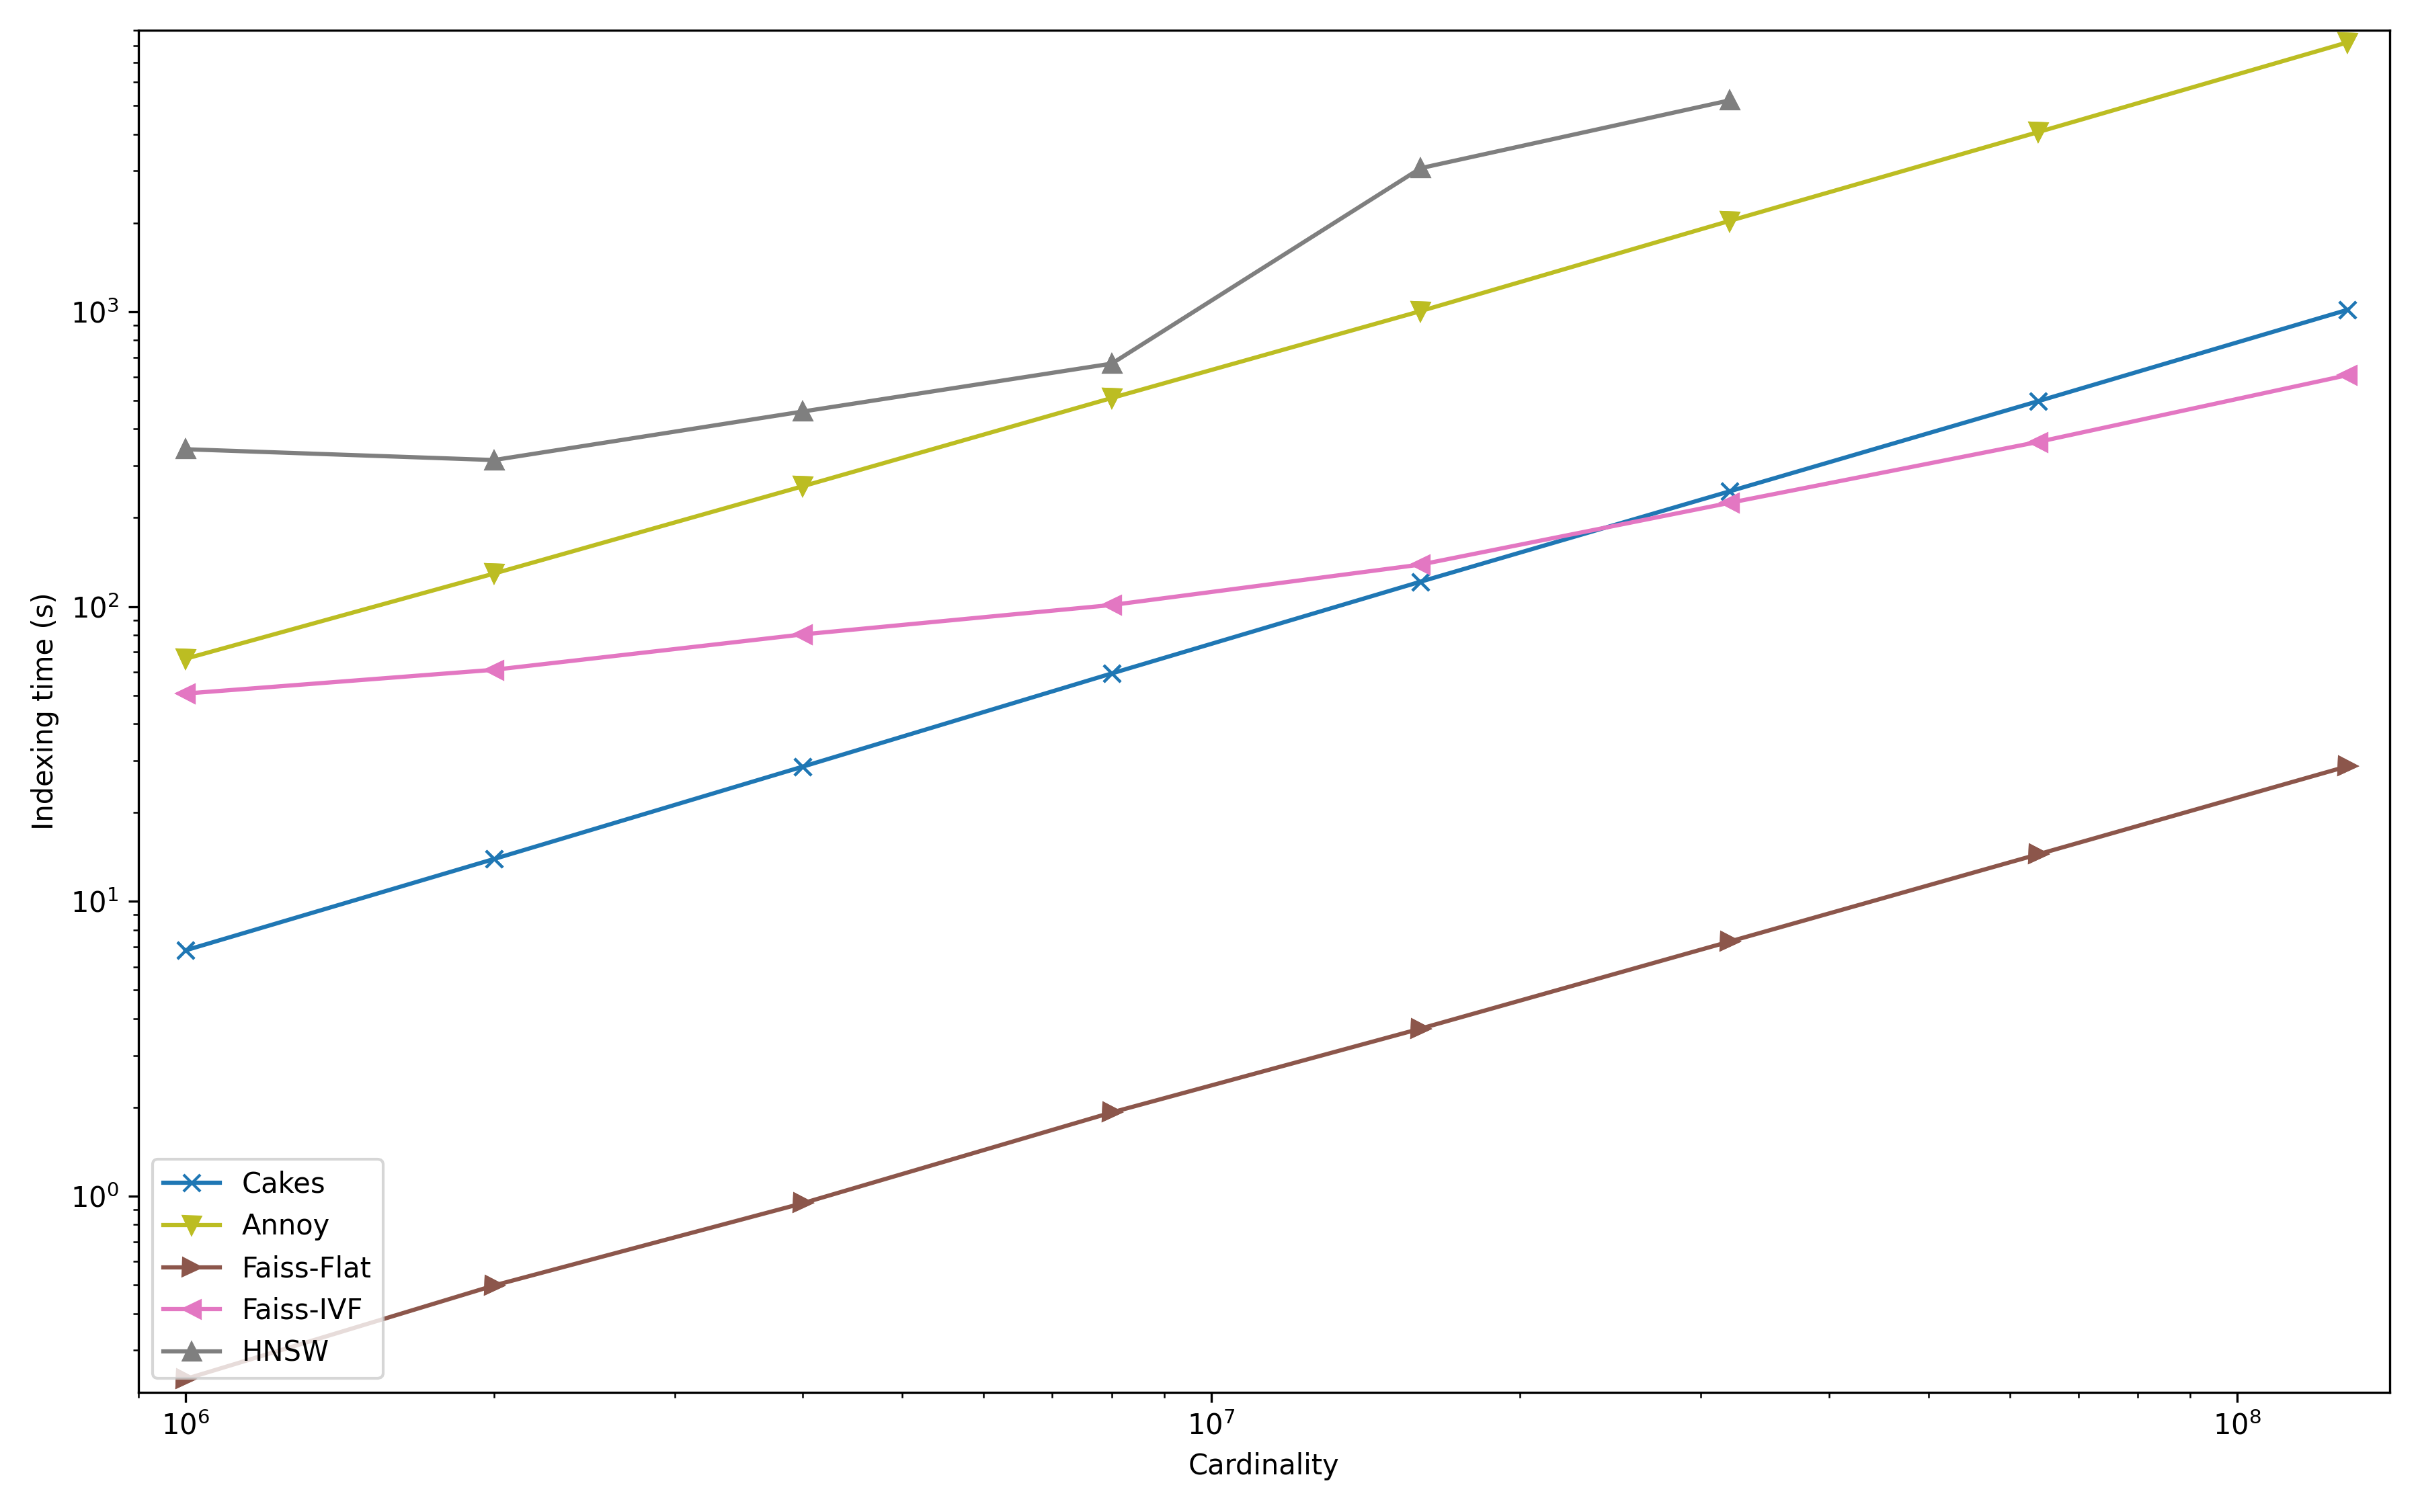
\includegraphics[width=0.95\textwidth]{plots/sift-indexing.png}\\
        \subcaption{Sift}
        \label{fig:results:sift-indexing}
    \end{subfigure}%
    \begin{subfigure}[b]{0.47\textwidth}
        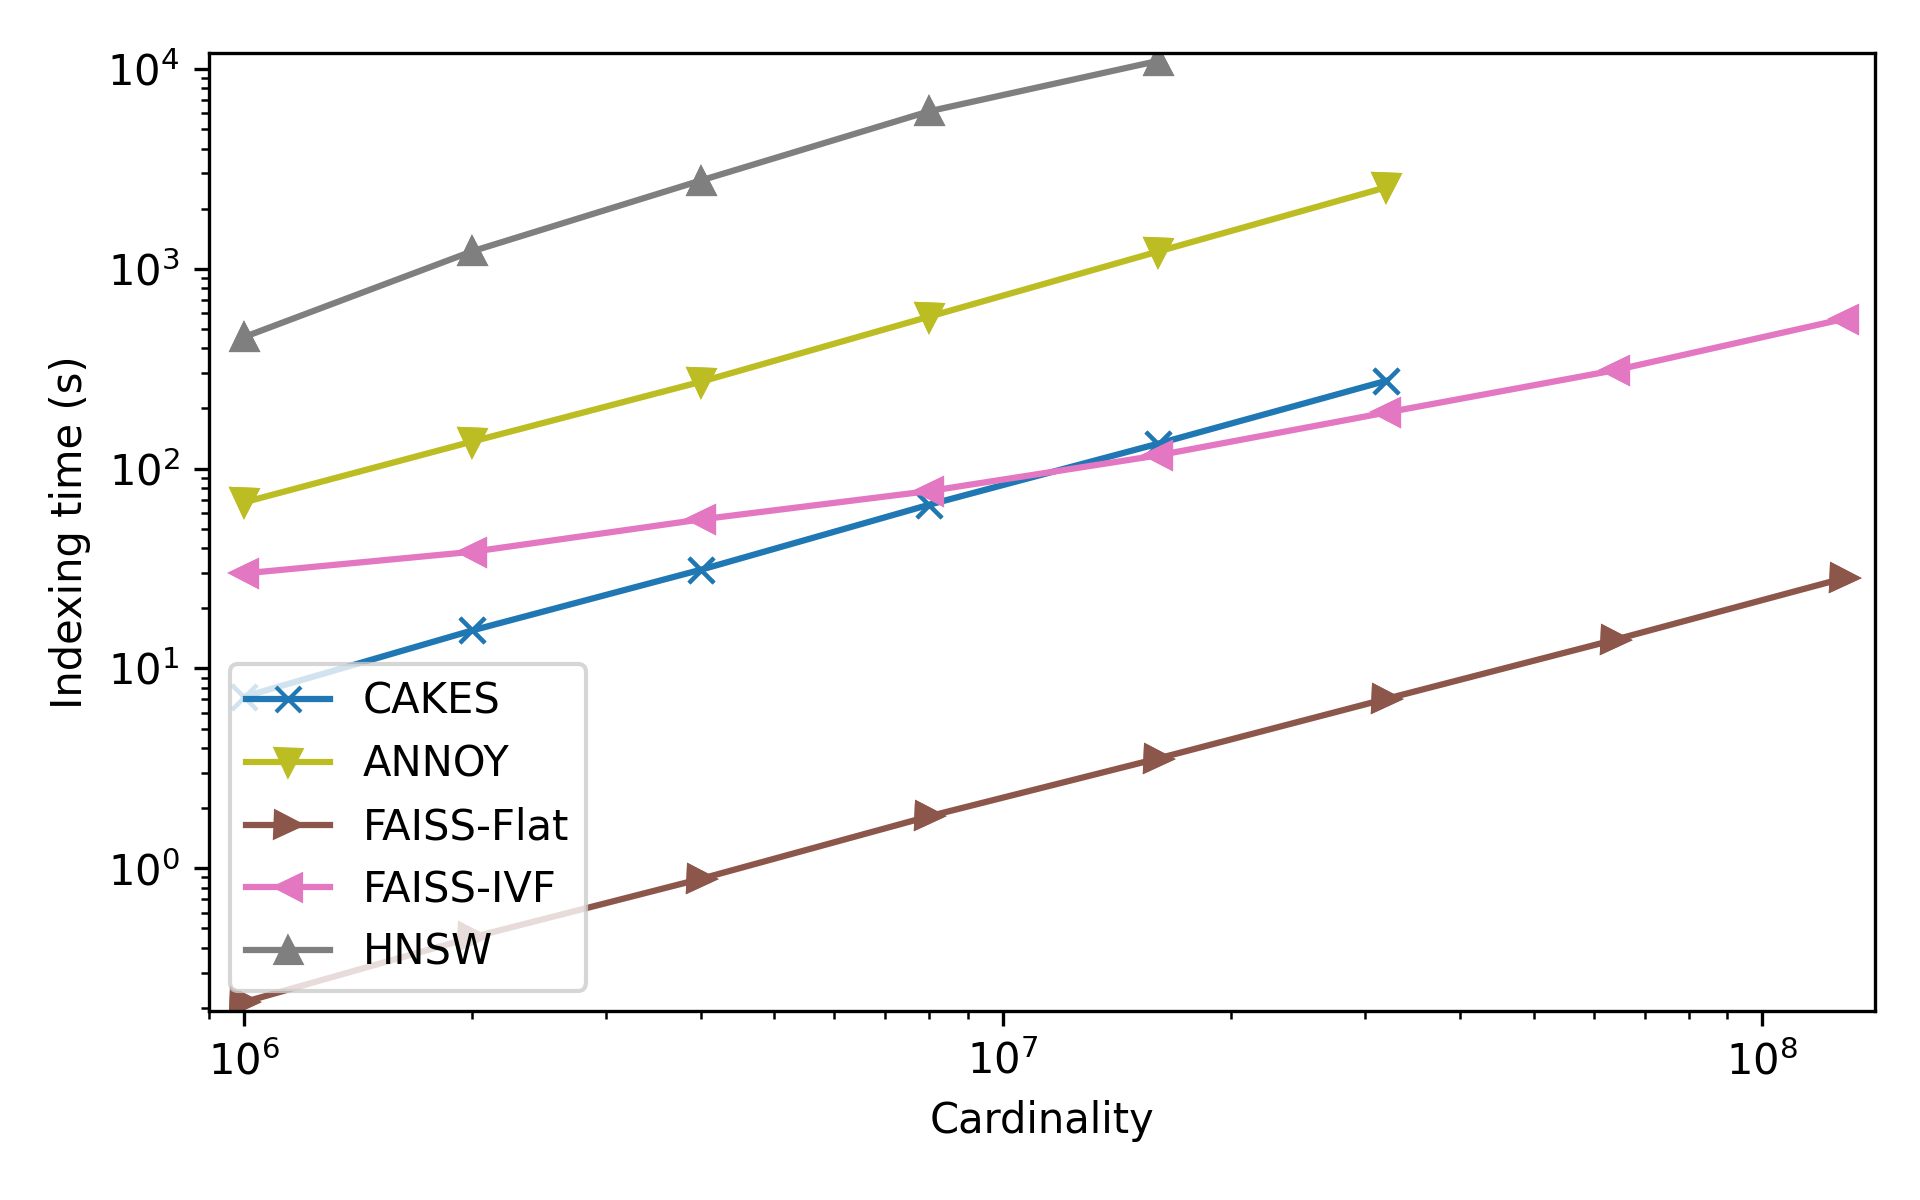
\includegraphics[width=0.95\textwidth]{plots/random-indexing.png}\\
        \subcaption{Random}
        \label{fig:results:random-indexing}
    \end{subfigure}%
    \\
    \vspace{1em}
    \caption{Indexing and tuning time for each algorithm with each of the ANN benchmark datasets and the Random dataset.}
    \label{fig:results:indexing}
\end{figure}


\subsection{Scaling Behavior and Recall}
\label{sec:results:scaling-behavior-and-recall}

Figures~\ref{fig:results:fashion-mnist-scaling},~\ref{fig:results:glove-25-scaling},~and~\ref{fig:results:sift-scaling} show the scaling behavior of CAKES algorithms and existing algorithms on augmented versions of the following ANN-benchmark datasets:

\begin{itemize}
    \item Fashion-Mnist under Euclidean distance,
    \item Glove-25 under Cosine distance, and
    \item Sift under Euclidean distance.
\end{itemize}

Figure~\ref{fig:results:random-scaling} shows the scaling behavior of CAKES algorithms and existing algorithms on a completely randomly generated dataset with same cardinality and dimensionality as Sift (1 million points in 128 dimensions).
Figures~\ref{fig:results:silva-scaling} and ~\ref{fig:results:radioml-scaling} show the scaling behavior of CAKES on Silva and RadioML respectively.
For these datasets, we took random sub-samples of the full datasets instead of augmenting them to higher cardinalities.

The horizontal axis in each figure shows the cardinality of the augmented dataset with synthetic points (see Section \ref{sec:methods:synthetic-data}).
The left-most point on each line is at the cardinality of the original dataset without any synthetic augmentation..
The vertical axis denotes throughput in queries per second.
Both axes are on a logarithmic scale.
In this section, we report results only for $k$-NN search with $k = 10$, but similar plots for $k = 100$ can be found in the Supplement.
For HNSW and ANNOY, we report the recall for each measurement in the plots. For algorithms which exhibit recall greater than $0.9995$, we do not report the recall in the plots, but we do report it in the tables below.

Table~\ref{tab:results:qps-and-recall} show the throughput and recall of CAKES's algorithms at each augmented cardinality for Fashion-Mnist, Glove-25, Sift, and Random. 
Though the plots in Figure~\ref{fig:results:scaling-plots} present results for each of CAKES's three algorithms separately, the results in the CAKES column in these tables represent the fastest CAKES algorithm at that dataset and cardinality only.
We used our auto-tuning approach (see Section~\ref{sec:methods:auto-tuning}) for each new tree (i.e. at each cardinality), and this approach was always able to select the fastest algorithm for each dataset at each cardinality.
Since we also allow for tuning hyper-parameters for the other algorithms, and we allow for different sets of hyper-parameters at each cardinality, it is a fair comparison for these tables to only list the performance of the tuned CAKES algorithm.
When reporting recall, we use $1.000*$ to denote that the recall is imperfect, but rounds to $1.000$ when we consider only three decimal places.


Figure~\ref{fig:results:scaling-plots} shows that for Fashion-Mnist, Glove-25, and Sift, as cardinality increases, the CAKES algorithms (Depth-First Sieve in blue, Repeated $\rho$-NN in green, and Breadth-First Sieve in purple) become faster than our Rust implementation of na\"{i}ve linear search (in orange).
Though we observe this trend, we note that the exact cardinality at which CAKES's algorithms overtake linear search differs by dataset. For Fashion-Mnist, CAKES begins exhibiting sub-linear performance starting at a cardinality near $10^5$, while for Glove-25 and Sift, this happens near $10^6$ and $10^7$ respectively. 
Which one of the three CAKES algorithms is fastest also differs by dataset.
For Fashion-Mnist, Depth-First Sieve is consistently fastest, while for Glove-25, the fastest is Repeated $\rho$-NN, and for Sift, Breadth-First Sieve. 
Additionally, on all three datasets, Depth-First Sieve and Breadth-First Sieve appear to have performance which is \emph{constant} in the cardinality of the dataset. 
With Glove-25, Repeated $\rho$-NN exhibits similar constant scaling. 
We also observe that on these three datasets, for nearly all cardinalities, all three of the CAKES algorithms are faster than FAISS-Flat (in brown), and that at some cardinality, CAKES's algorithms become faster than FAISS-IVF (in pink). 
For Fashion-Mnist, CAKES becomes faster than FAISS-IVF near cardinality $10^5$, whereas for Glove-25 and Sift, this happens near cardinality $10^7$. 
On all three of these datasets, HNSW (in gray) and ANNOY (in yellow) are faster than CAKES's algorithms for all cardinalities; however, CAKES exhibits perfect or near-perfect recall on each dataset, while HNSW and ANNOY exhibit much lower recall, as shown in Table~\ref{tab:datasets:summary}.
While recall for CAKES's algorithms does not degrade with cardinality, recall for HNSW and ANNOY does degrade with cardinality. 
At a cardinality multiplier as low as eight, HNSW and ANNOY have recall of $0.525$ and $0.857$ respectively for Fashion-Mnist, 0.607 and 0.832 for Glove-25, and 0.782 and 0.686 on Sift. 
In contrast, CAKES has perfect recall on Fashion-Mnist and Sift (because the distance function used with these datasets is a metric), and near-perfect recall on Glove-25 (because the Cosine distance function is not a metric).


In contrast with the results on the ANN Benchmark datasets reported above, with the Random dataset, as seen in Figure~\ref{fig:results:random-scaling}, we observe that the three CAKES algorithms are the slowest out of all algorithms, at all cardinalities.
As with the real datasets, HNSW and ANNOY are the fastest algorithms, and CAKES exhibits perfect recall at all cardinalities.
HNSW and ANNOY exhibit \emph{much} lower recall on this random dataset than on any of the ANN benchmark datasets;
in particular, with a multiplier of 1, HNSW and ANNOY have recall as low as 0.060 and 0.028 respectively, as reported in Table~\ref{tab:results:random}.

For Silva and RadioML, we benchmarked only CAKES's algorithms because none HNSW, ANNOY or FAISS support neither the required distance functions nor, in the case of RadioML, complex-valued data.
Due to the massive sizes of these datasets, we took random sub-samples of the dataset with lower cardinalities for our benchmarks, rather than augmented versions of the dataset.
With Silva, as shown in Figure~\ref{fig:results:silva-scaling}, we observe that for all algorithms, throughput seems to linearly decrease as cardinality increases, but that it seems to begin levelling off near cardinality $10^5$.
Until cardinality near $10^4$, Depth-First Sieve is the fastest CAKES algorithm, but for larger cardinalities, Repeated $\rho$-NN is the fastest CAKES algorithm.
For RadioML, as shown in Figure~\ref{fig:results:radioml-scaling}, we observe that throughput declines nearly linearly the three CAKES algorithms exhibit nearly indistinguishable performance for all cardinalities.
In particular, throughput of CAKES algorithms is identical within three significant figures for all cardinalities.

\begin{figure}
    \begin{subfigure}[b]{0.47\textwidth}
        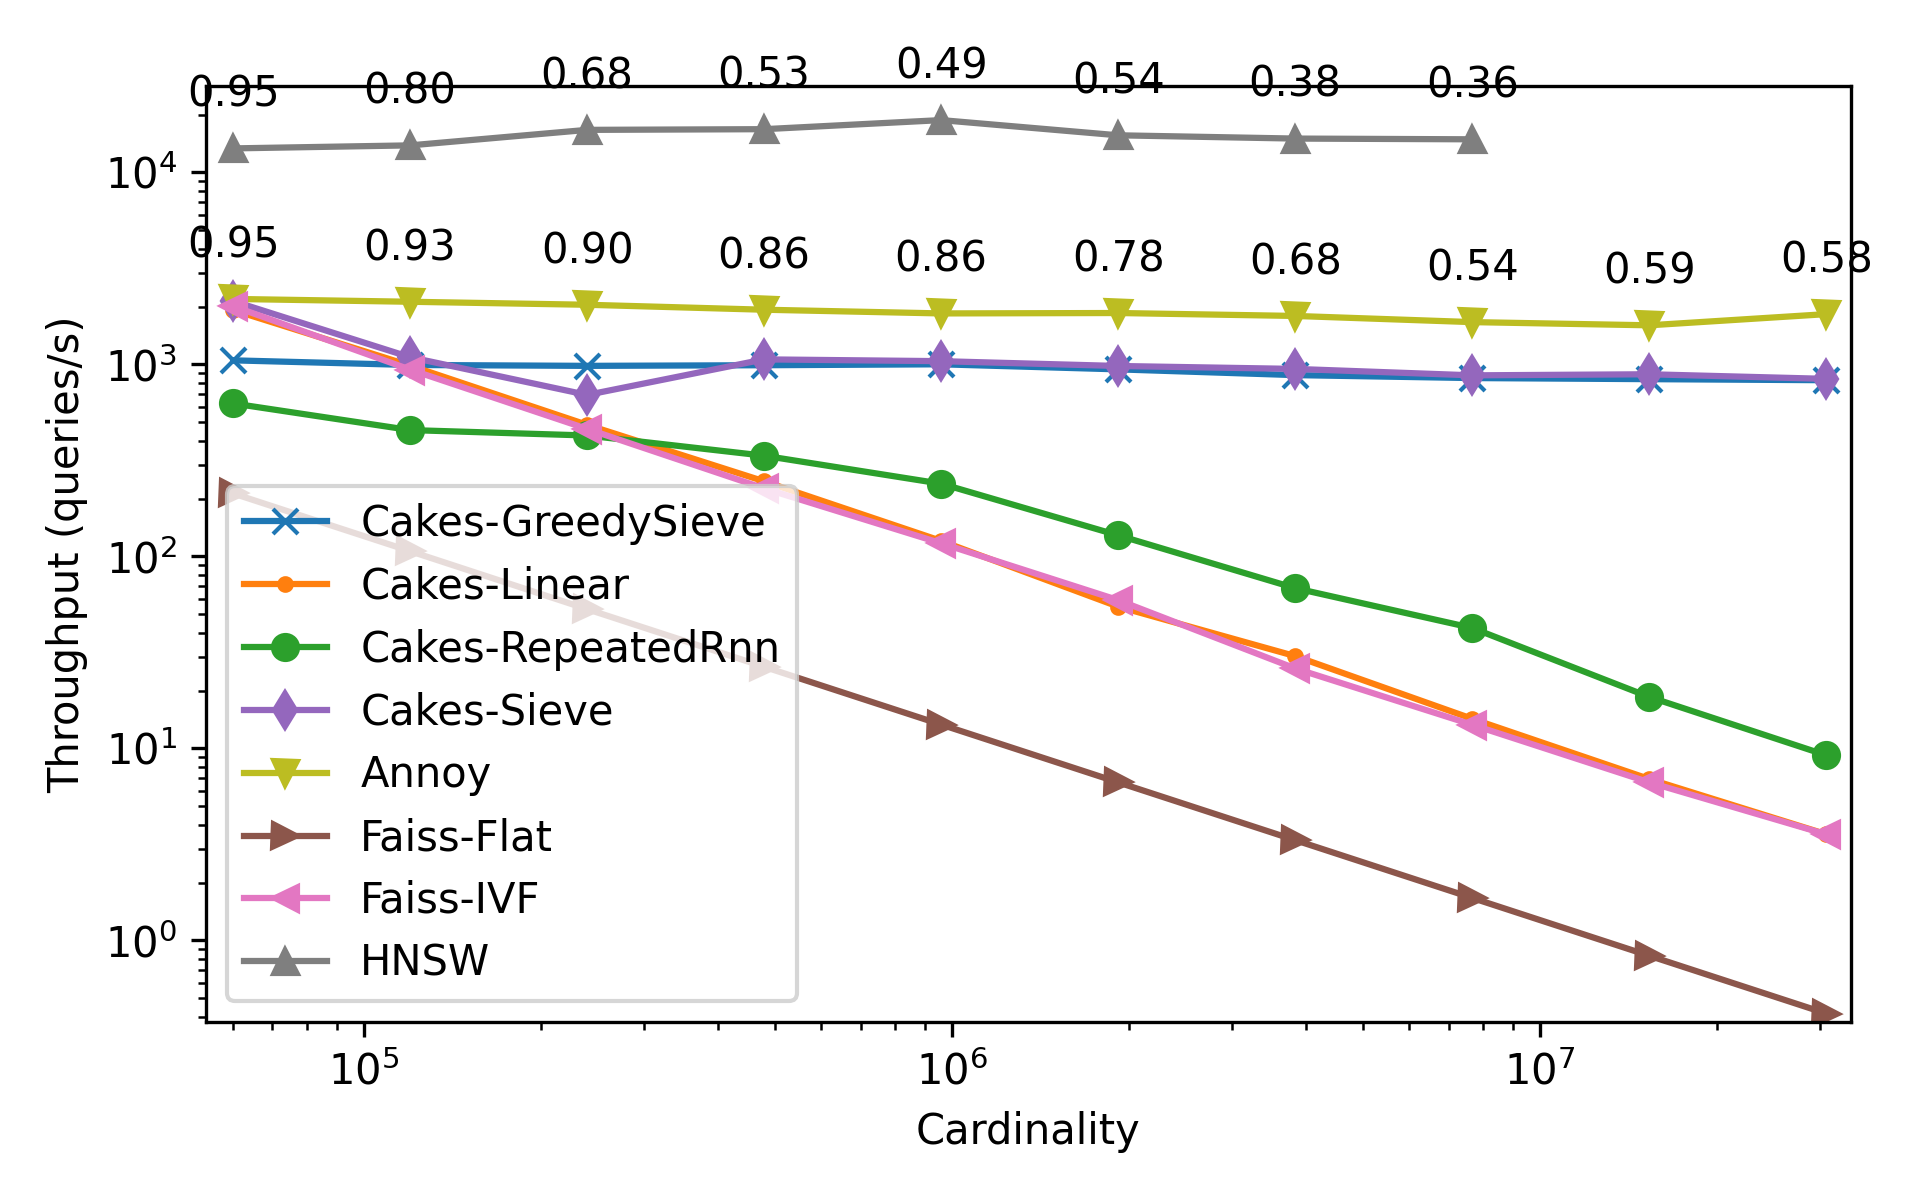
\includegraphics[width=0.95\textwidth]{plots/fashion-mnist-knn-10.png}
        \subcaption{Fashion-Mnist for $k=10$.}
        \label{fig:results:fashion-mnist-scaling}
    \end{subfigure}%
    \begin{subfigure}[b]{0.47\textwidth}
        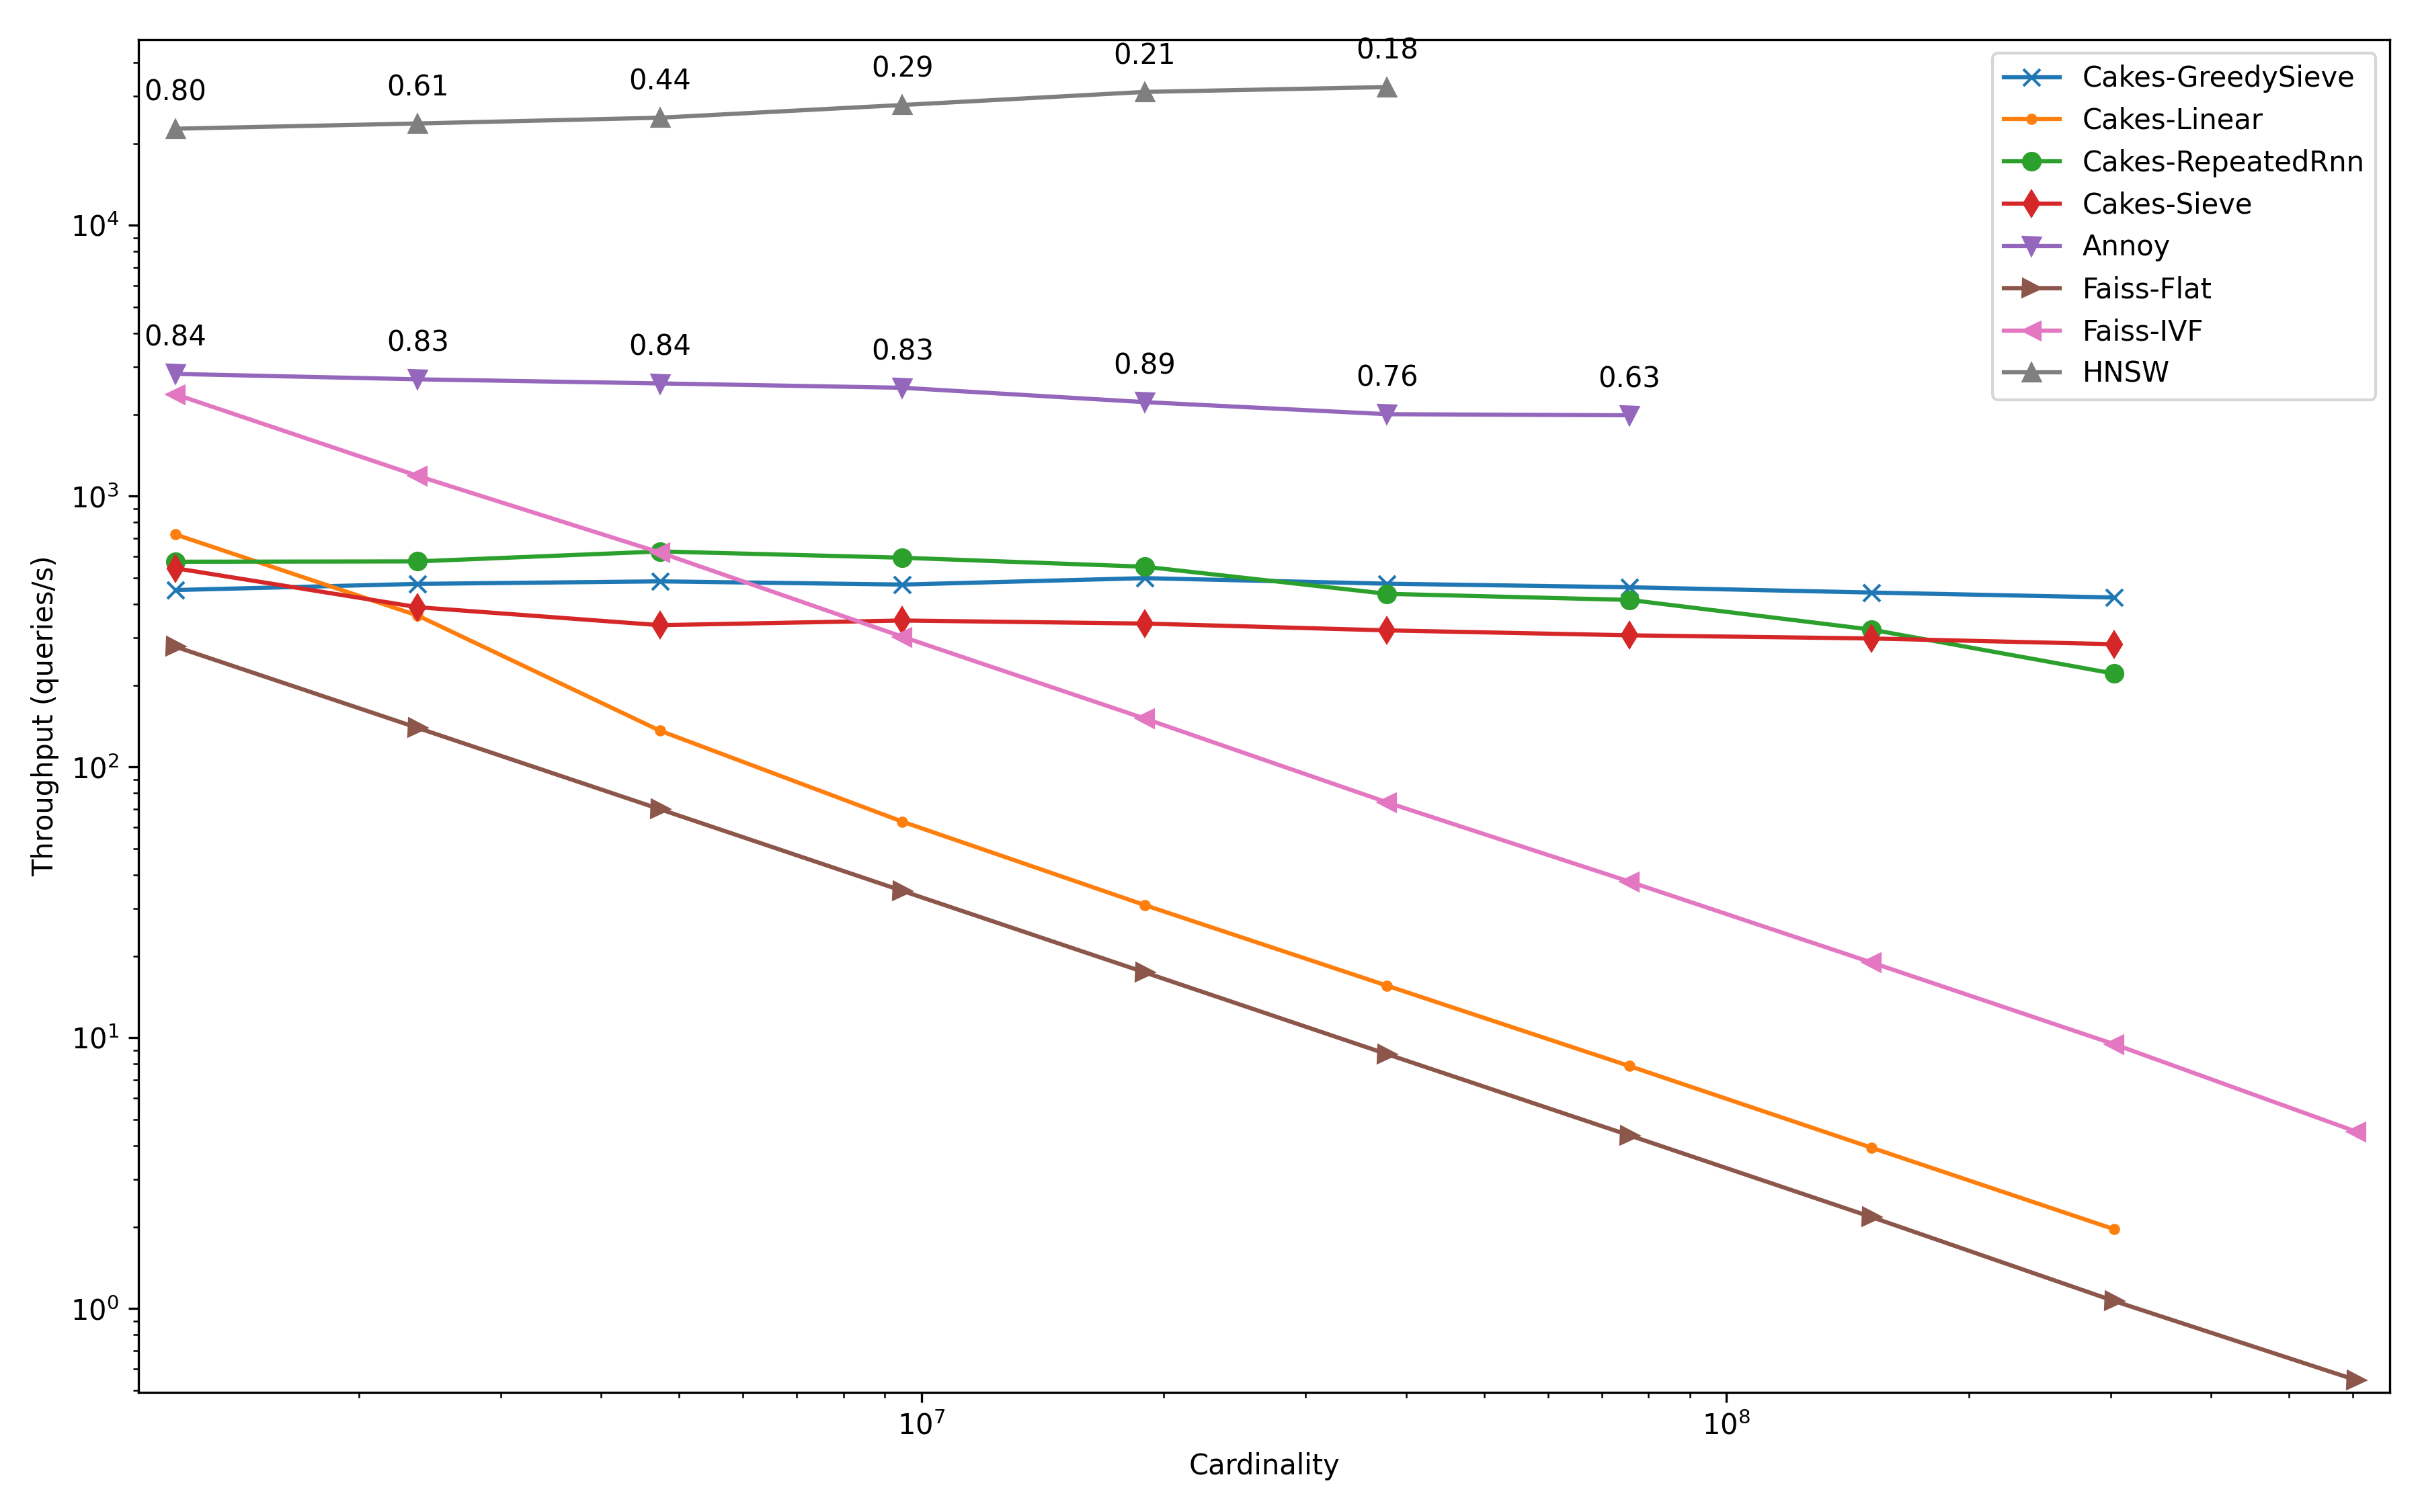
\includegraphics[width=0.95\textwidth]{plots/glove-25-knn-10.png}
        \subcaption{Glove-25 for $k=10$.}
        \label{fig:results:glove-25-scaling}
    \end{subfigure}%
    \vspace{1em}
    \\
    \begin{subfigure}[b]{0.47\textwidth}
        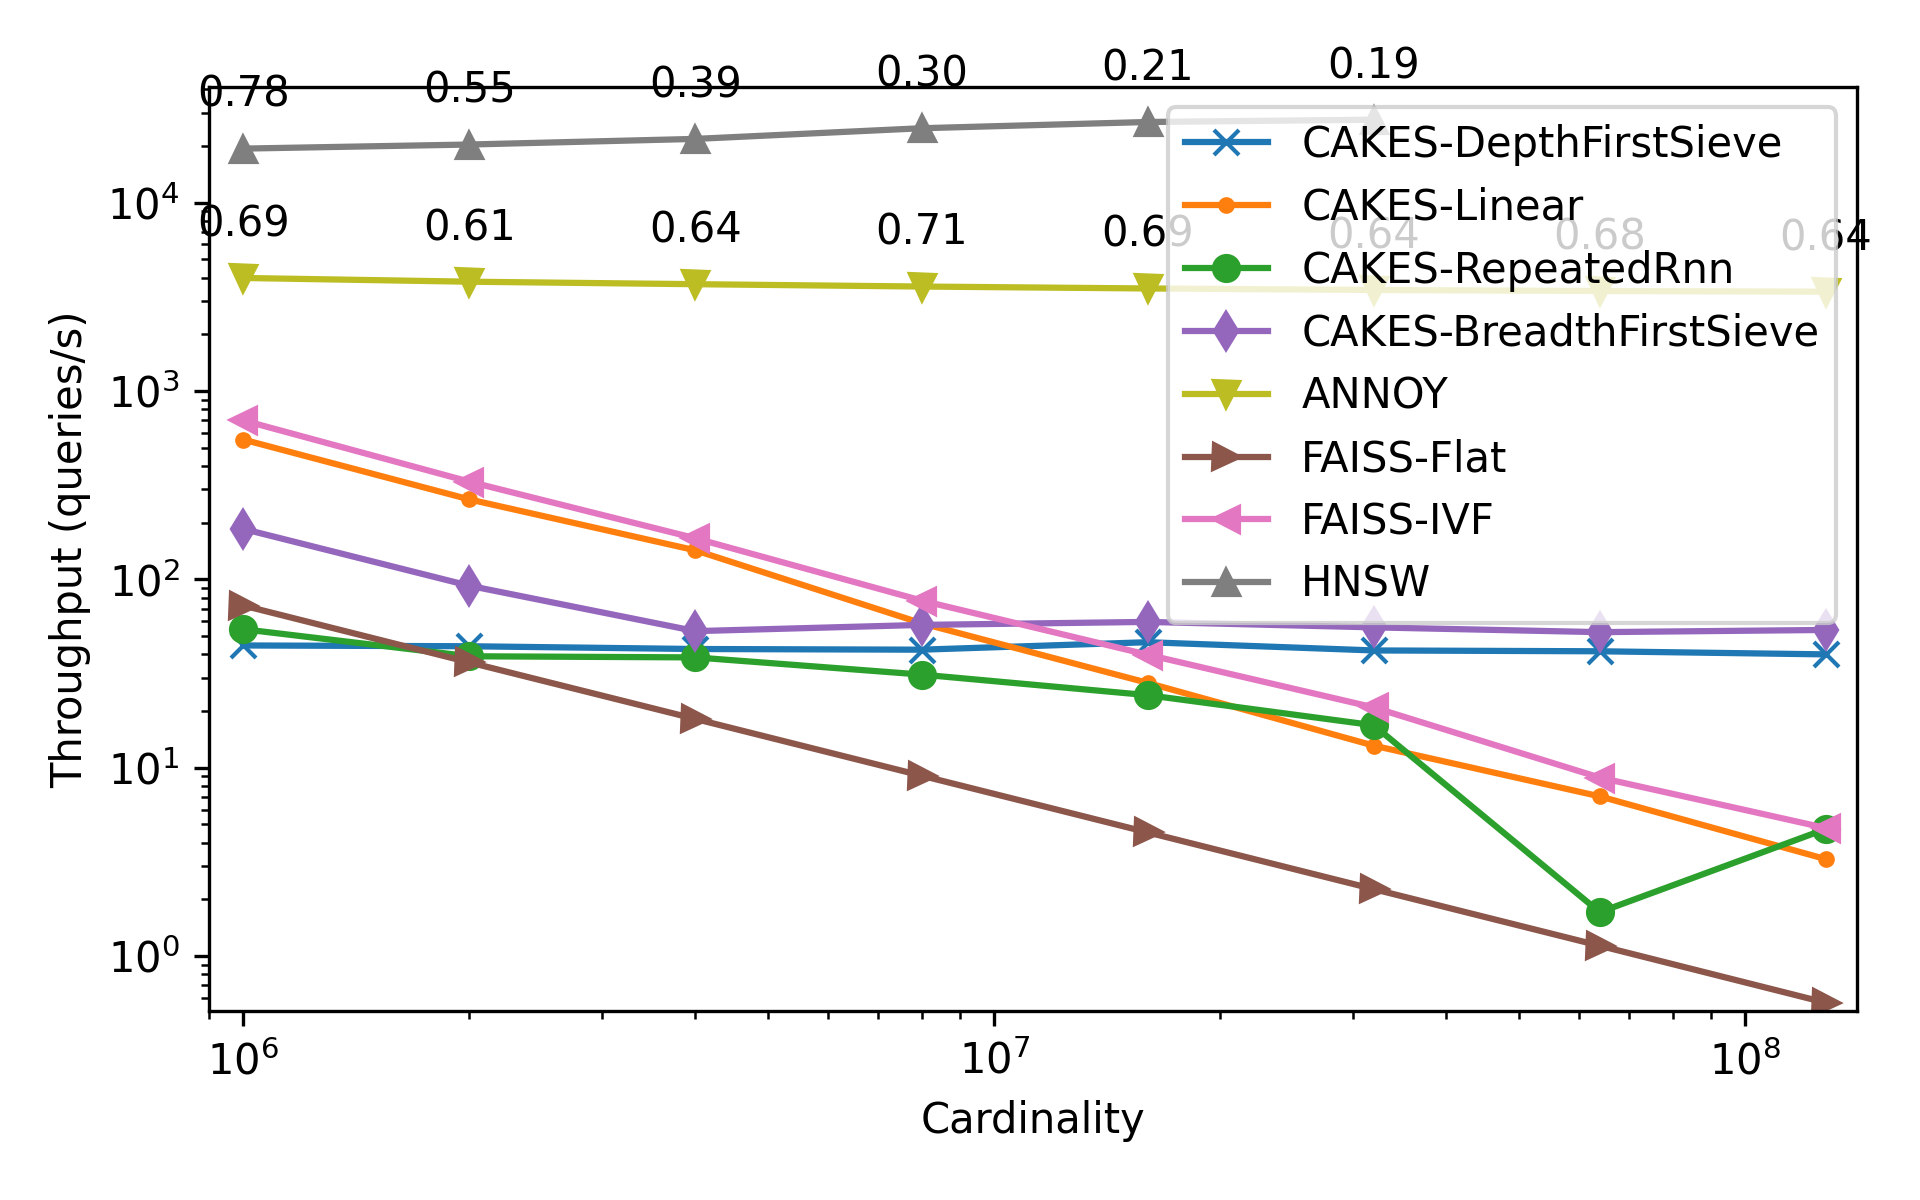
\includegraphics[width=0.95\textwidth]{plots/sift-knn-10.png}
        \subcaption{Sift for $k=10$.}
        \label{fig:results:sift-scaling}
    \end{subfigure}%
    \begin{subfigure}[b]{0.47\textwidth}
        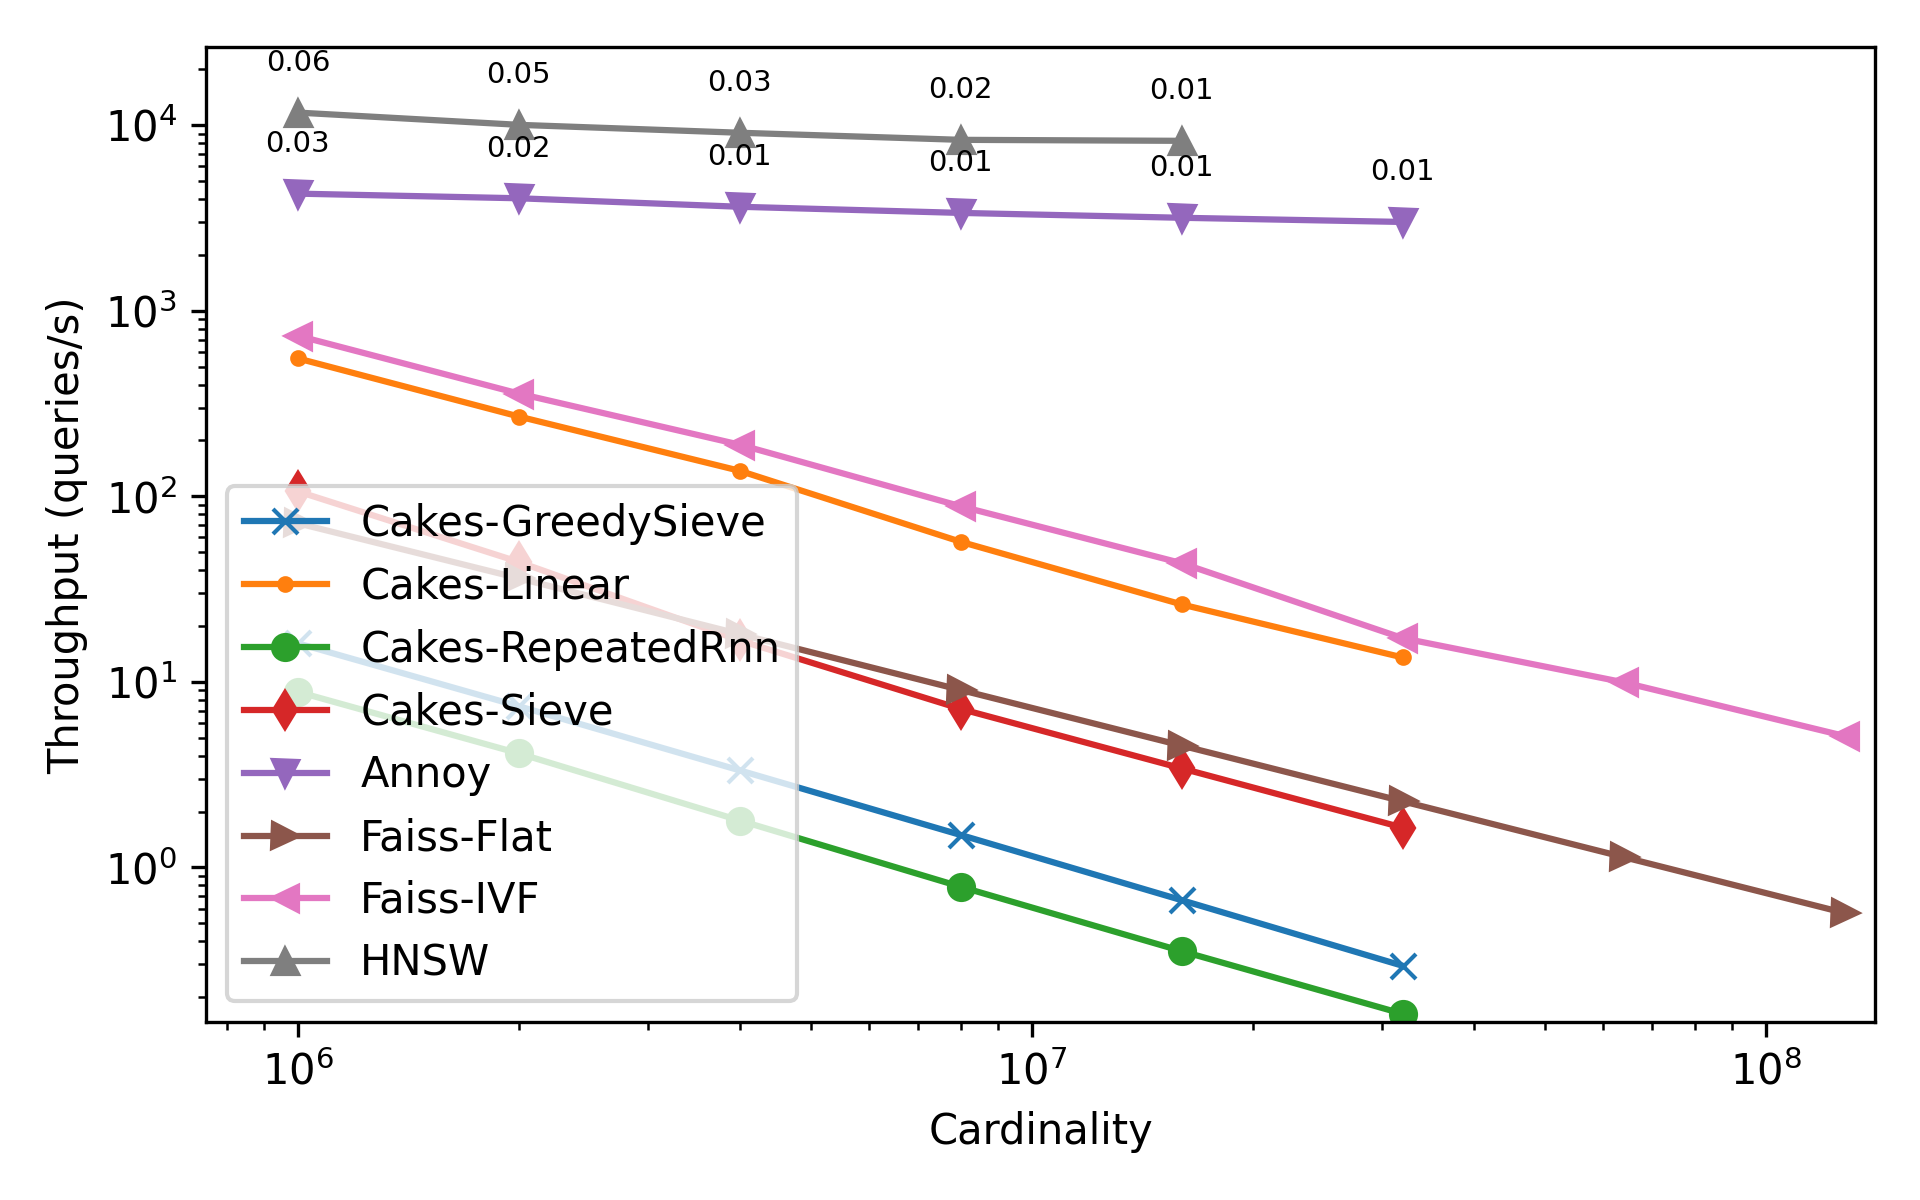
\includegraphics[width=0.95\textwidth]{plots/radio-ml-knn-10.png}
        \subcaption{RadioML for $k=10$ at SnR = 10dB.}
        \label{fig:results:radioml-scaling}
    \end{subfigure}%
    \vspace{1em}
    \\
    \begin{subfigure}[b]{0.47\textwidth}
        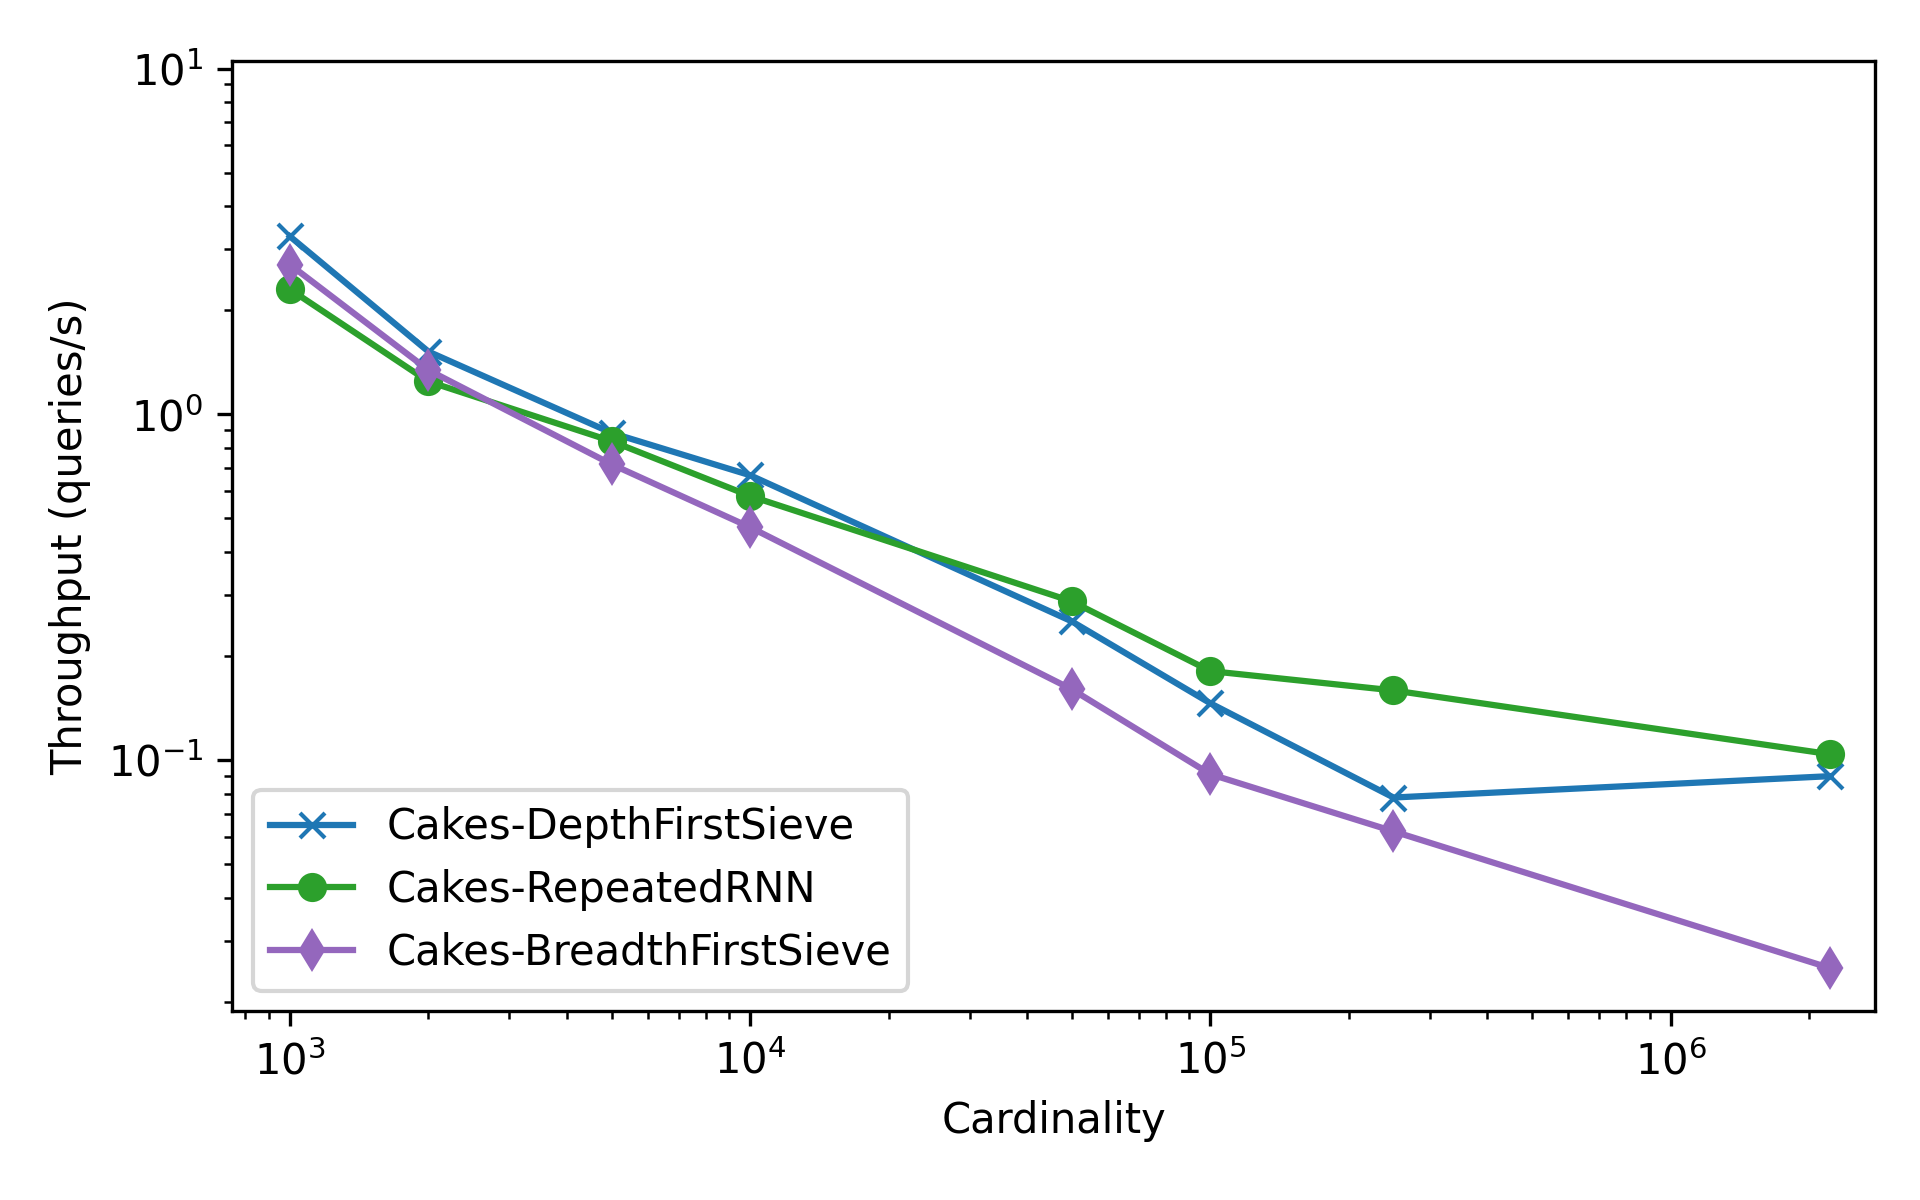
\includegraphics[width=0.95\textwidth]{plots/silva-knn-10.png}
        \subcaption{Silva for $k=10$.}
        \label{fig:results:silva-scaling}
    \end{subfigure}%
    \begin{subfigure}[b]{0.47\textwidth}
        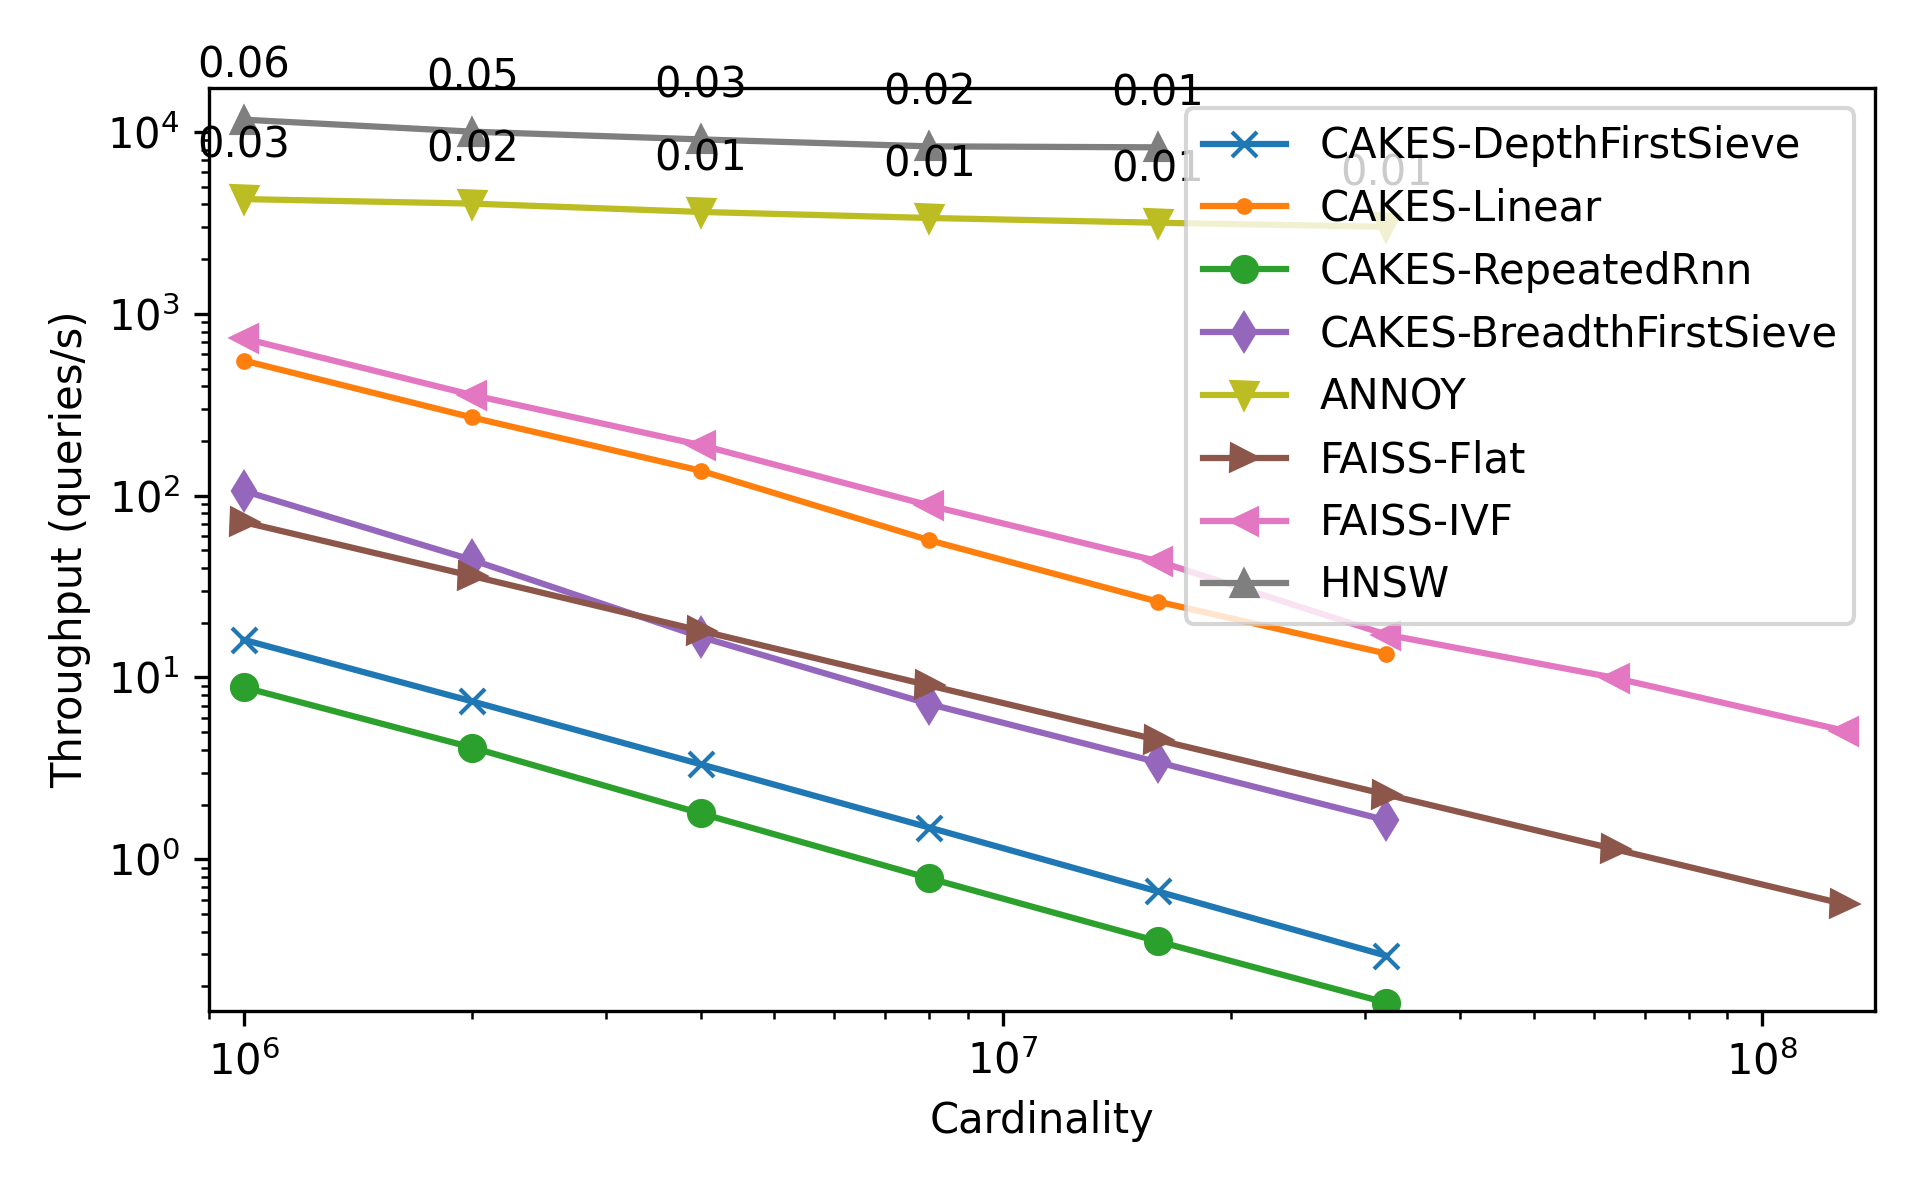
\includegraphics[width=0.95\textwidth]{plots/random-knn-10.png}
        \subcaption{A random dataset for $k=10$.}
        \label{fig:results:random-scaling}
    \end{subfigure}%
    \caption{Throughput across six datasets, including a randomly-generated dataset.
    In each plot, the horizontal axis represents increasing cardinality of the dataset, while the vertical axis represents the throughput in queries per second (higher is better).
    For some algorithms, we were not able to take measurements for each cardinality because the index-building required more RAM than was available (i.e. more then 512GB).}
    \label{fig:results:scaling-plots}
\end{figure}


\begin{table*}[h]
    % \renewcommand{\arraystretch}{1.15}
    \caption{QPS (queries per second) and Recall vs naive linear search on the Fashion-Mnist, Glove-25, Sift and Random datasets.
    A recall value of $1.000*$ denotes imperfect recall that rounds to 1.000.}
    \label{tab:results:qps-and-recall}
    \vskip 0.15in
    \begin{center}
        \begin{small}
            \begin{sc}
                \begin{tabular}{|c|l|p{1.2cm}|p{0.8cm}|p{1.2cm}|p{0.8cm}|p{1.2cm}|p{0.8cm}|p{1.2cm}|p{0.8cm}|}
                    \hline
                    & \multirow{2}{*}{\textbf{Multiplier}} & \multicolumn{2}{|c}{\textbf{hnsw}} & \multicolumn{2}{|c}{\textbf{annoy}} & \multicolumn{2}{|c}{\textbf{faiss-ivf}}  & \multicolumn{2}{|c|}{\textbf{cakes}} \\\cline{3-10}
                    & & QPS & Recall & QPS & Recall & QPS & Recall & QPS & Recall \\\cline{2-10}
                    \hline
                    \hline
                    \multirow{10}{*}{\rotatebox[origin=c]{90}{\textbf{Fashion-Mnist}}}
                    & 1   & 1.33~$\times10^{4}$ & 0.954  & 2.19~$\times10^{3}$ & 0.950  & 2.01~$\times10^{3}$ & 1.000* & 2.17~$\times10^{3}$ & 1.000  \\\cline{2-10}
                    & 2   & 1.38~$\times10^{4}$ & 0.803  & 2.12~$\times10^{3}$ & 0.927  & 9.39~$\times10^{2}$ & 1.000* & 1.14~$\times10^{3}$ & 1.000  \\\cline{2-10}
                    & 4   & 1.66~$\times10^{4}$ & 0.681  & 2.04~$\times10^{3}$ & 0.898  & 4.61~$\times10^{2}$ & 0.997  & 9.82~$\times10^{2}$ & 1.000  \\\cline{2-10}
                    & 8   & 1.68~$\times10^{4}$ & 0.525  & 1.93~$\times10^{3}$ & 0.857  & 2.26~$\times10^{2}$ & 0.995  & 1.18~$\times10^{3}$ & 1.000  \\\cline{2-10}
                    & 16  & 1.87~$\times10^{4}$ & 0.494  & 1.84~$\times10^{3}$ & 0.862  & 1.17~$\times10^{2}$ & 0.991  & 1.20~$\times10^{3}$ & 1.000  \\\cline{2-10}
                    & 32  & 1.56~$\times10^{4}$ & 0.542  & 1.85~$\times10^{3}$ & 0.775  & 5.91~$\times10^{1}$ & 0.985  & 1.16~$\times10^{3}$ & 1.000  \\\cline{2-10}
                    & 64  & 1.50~$\times10^{4}$ & 0.378  & 1.78~$\times10^{3}$ & 0.677  & 2.61~$\times10^{1}$ & 0.968  & 1.10~$\times10^{3}$ & 1.000  \\\cline{2-10}
                    & 128 & 1.49~$\times10^{4}$ & 0.357  & 1.66~$\times10^{3}$ & 0.538  & 1.33~$\times10^{1}$ & 0.964  & 1.04~$\times10^{3}$ & 1.000  \\\cline{2-10}
                    & 256 & --                  & --     & 1.60~$\times10^{3}$ & 0.592  & 6.65~$\times10^{0}$ & 0.962  & 1.06~$\times10^{3}$ & 1.000  \\\cline{2-10}
                    & 512 & --                  & --     & 1.83~$\times10^{3}$ & 0.581  & 3.56~$\times10^{0}$ & 0.949  & 1.04~$\times10^{3}$ & 1.000  \\
                    \hline
                    \hline
                    \multirow{9}{*}{\rotatebox[origin=c]{90}{\textbf{Glove-25}}}
                    & 1   & 2.28~$\times10^{4}$ & 0.801 & 2.83~$\times10^{3}$ & 0.835 & 2.38~$\times10^{3}$ & 1.000* & 7.22~$\times10^{2}$ & 1.000* \\\cline{2-10}
                    & 2   & 2.38~$\times10^{4}$ & 0.607 & 2.70~$\times10^{3}$ & 0.832 & 1.19~$\times10^{3}$ & 1.000* & 5.75~$\times10^{2}$ & 1.000* \\\cline{2-10}
                    & 4   & 2.50~$\times10^{4}$ & 0.443 & 2.61~$\times10^{3}$ & 0.839 & 6.19~$\times10^{2}$ & 1.000* & 6.25~$\times10^{2}$ & 1.000* \\\cline{2-10}
                    & 8   & 2.78~$\times10^{4}$ & 0.294 & 2.51~$\times10^{3}$ & 0.834 & 3.03~$\times10^{2}$ & 1.000* & 5.93~$\times10^{2}$ & 1.000* \\\cline{2-10}
                    & 16  & 3.11~$\times10^{4}$ & 0.213 & 2.23~$\times10^{3}$ & 0.885 & 1.51~$\times10^{2}$ & 1.000* & 5.49~$\times10^{2}$ & 1.000* \\\cline{2-10}
                    & 32  & 3.24~$\times10^{4}$ & 0.178 & 2.01~$\times10^{3}$ & 0.764 & 7.40~$\times10^{1}$ & 0.999  & 4.75~$\times10^{2}$ & 1.000* \\\cline{2-10}
                    & 64  & --                  & --    & 1.99~$\times10^{3}$ & 0.631 & 3.77~$\times10^{1}$ & 0.997  & 4.61~$\times10^{2}$ & 1.000* \\\cline{2-10}
                    & 128 & --                  & --    & --                  & --    & 1.90~$\times10^{1}$ & 0.998  & 4.41~$\times10^{2}$ & 1.000* \\\cline{2-10}
                    & 256 & --                  & --    & --                  & --    & 9.47~$\times10^{0}$ & 0.998  & 4.23~$\times10^{2}$ & 1.000* \\
                    \hline
                    \hline
                    \multirow{8}{*}{\rotatebox[origin=c]{90}{\textbf{Sift}}}
                    & 1   & 1.93~$\times10^{4}$ & 0.782 & 3.98~$\times10^{3}$ & 0.686 & 6.98~$\times10^{2}$ & 1.000* & 5.52~$\times10^{2}$ & 1.000 \\\cline{2-10}
                    & 2   & 2.03~$\times10^{4}$ & 0.552 & 3.80~$\times10^{3}$ & 0.614 & 3.30~$\times10^{2}$ & 1.000* & 2.66~$\times10^{2}$ & 1.000 \\\cline{2-10}
                    & 4   & 2.18~$\times10^{4}$ & 0.394 & 3.69~$\times10^{3}$ & 0.637 & 1.65~$\times10^{2}$ & 1.000* & 1.43~$\times10^{2}$ & 1.000 \\\cline{2-10}
                    & 8   & 2.48~$\times10^{4}$ & 0.298 & 3.58~$\times10^{3}$ & 0.710 & 7.72~$\times10^{1}$ & 1.000* & 7.94~$\times10^{1}$ & 1.000 \\\cline{2-10}
                    & 16  & 2.68~$\times10^{4}$ & 0.210 & 3.50~$\times10^{3}$ & 0.690 & 3.98~$\times10^{1}$ & 1.000* & 8.12~$\times10^{1}$ & 1.000 \\\cline{2-10}
                    & 32  & 2.75~$\times10^{4}$ & 0.193 & 3.44~$\times10^{3}$ & 0.639 & 2.09~$\times10^{1}$ & 0.999  & 7.81~$\times10^{1}$ & 1.000 \\\cline{2-10}
                    & 64  & --                  & --    & 3.39~$\times10^{3}$ & 0.678 & 8.87~$\times10^{0}$ & 0.997  & 7.43~$\times10^{1}$ & 1.000 \\\cline{2-10}
                    & 128 & --                  & --    & 3.36~$\times10^{3}$ & 0.643 & 4.78~$\times10^{0}$ & 0.993  & 6.80~$\times10^{1}$ & 1.000 \\
                    \hline
                    \hline
                    \multirow{6}{*}{\rotatebox[origin=c]{90}{\textbf{Random}}}
                    & 1  & 1.17~$\times10^{4}$ & 0.060 & 4.28~$\times10^{3}$ & 0.028 & 7.34~$\times10^{2}$ & 1.000* & 5.54~$\times10^{2}$ & 1.000 \\\cline{2-10}
                    & 2  & 1.01~$\times10^{4}$ & 0.048 & 4.04~$\times10^{3}$ & 0.021 & 3.58~$\times10^{2}$ & 1.000* & 2.69~$\times10^{2}$ & 1.000 \\\cline{2-10}
                    & 4  & 9.12~$\times10^{3}$ & 0.031 & 3.64~$\times10^{3}$ & 0.014 & 1.90~$\times10^{2}$ & 1.000* & 1.37~$\times10^{2}$ & 1.000 \\\cline{2-10}
                    & 8  & 8.35~$\times10^{3}$ & 0.022 & 3.37~$\times10^{3}$ & 0.013 & 8.84~$\times10^{1}$ & 1.000* & 5.69~$\times10^{1}$ & 1.000 \\\cline{2-10}
                    & 16 & 8.25~$\times10^{3}$ & 0.008 & 3.17~$\times10^{3}$ & 0.006 & 4.36~$\times10^{1}$ & 1.000* & 2.61~$\times10^{1}$ & 1.000 \\\cline{2-10}
                    & 32 & --                  & --    & 3.01~$\times10^{3}$ & 0.007 & 1.72~$\times10^{1}$ & 1.000* & 1.35~$\times10^{1}$ & 1.000 \\
                    \hline
                \end{tabular}
            \end{sc}
        \end{small}
    \end{center}
    \vskip -0.1in
\end{table*}
